%%   =========================
%%   |     Master Thesis     |
%%   =========================
%%
%%    Author: Romain Liautaud <romain@liautaud.fr>
%%     Tutor: Clément Pascutto <clement@tarides.org>
%%   Subject: Garbage collection of a decentralized data store.
%%   Company: Tarides <contact@tarides.org>

\documentclass[11pt]{article}

% Configuration files (packages and definitions).
%% Global configuration for the document.

\usepackage[a4paper, margin=0.7in, bottom=.8in]{geometry}
\usepackage{graphicx}
\usepackage{svg}
\usepackage{minted}
\usepackage{stmaryrd}
\usepackage[english]{babel}
\usepackage{lmodern}
\usepackage{mathpazo}
\usepackage[T1]{fontenc}
\usepackage{fontspec}
\usepackage{caption}
\usepackage{subcaption}
\usepackage{fancyvrb}
\usepackage{amssymb}
\usepackage{amsmath}
\usepackage{amsthm}
\usepackage[colorlinks, allcolors=gray]{hyperref}
\usepackage[noabbrev, capitalize, nameinlink]{cleveref}
\usepackage{algorithm}
\usepackage[noend]{algpseudocode}
\usepackage{titlesec}
\usepackage[pdf]{graphviz}
\usepackage{titling}
\usepackage{enumitem}
\usepackage{tabu}
\usepackage{appendix}
\usepackage{tikz}
\usetikzlibrary{shapes,arrows}

% Pseudocode listigs.
\usepackage{listings}
\lstset{basicstyle=\footnotesize\ttfamily,breaklines=true,mathescape}

% Typography
\usepackage[scaled=1,osf,tighter]{newpxtext}
\setsansfont{Latin Modern Sans}
\renewcommand*{\ttdefault}{npxtt}

% Minted styling
\usemintedstyle{tango}
\setminted{linenos}
\setminted{fontsize=\small}
\setminted{xleftmargin=2em}
\setminted{baselinestretch=.98}

% Custom figure captions
\DeclareCaptionFormat{customcap}{%
  \vspace{0.5em}%
  \linebreak%
  \setlength{\fboxsep}{4pt}%
  \colorbox{black!4}{%
    \hspace{-0.1em}%
    \parbox{0.98\linewidth}{%
      \centering\textit{#1}#2#3}}%
\vspace{0.5em}}%
\captionsetup[figure]{format=customcap}

% Figure margins
\setlength{\textfloatsep}{1.5em}
\setlength{\intextsep}{2em}

% Custom appendix captions
\newcommand{\colorsection}[1]{%
  \vspace{0.5em}%
  \linebreak%
  \setlength{\fboxsep}{6pt}%
  \colorbox{black!4}{%
    \parbox{\linewidth}{\centering \textit{Appendix~\thesection}:\ #1}}%
  \vspace{0.5em}}

% Highlight boxes
\def\highlightbox#1{%
  \setlength{\fboxsep}{2pt}
  \colorbox{yellow!60}{\textbf{#1}}}

% Appendix reference boxes
\def\appendixref#1{%
  \noindent%
  \setlength{\fboxsep}{6pt}%
  \colorbox{yellow!20}{%
    $\hspace{0.3em} \triangleright$%
    \hspace{0.2em}%
    \parbox{\linewidth-2.8em}{\textit{#1}}}}

% Title margins
\titlespacing*{\subsection}{0pt}{2\baselineskip}{\baselineskip}

% Line spread
\linespread{1.05}

% Algorithms formatting
\algrenewcommand\alglinenumber[1]{\footnotesize #1}
\algrenewcomment[1]{\(\triangleright\) #1}

% Circled numbers
\newcommand*\circled[1]{\tikz[baseline=(char.base)]{
    \node[shape=circle,draw,inner sep=2pt] (char) {#1};}}

% Subtitle definition
\newcommand*\subtitle[1]{\newcommand{\thesubtitle}{#1}}

% Credits definition
\newcommand*\credits[1]{\newcommand{\thecredits}{#1}}

% Abstract redefinition
\renewcommand\abstract[1]{\newcommand{\theabstract}{#1}}

% Theorems and definitions
\theoremstyle{definition}
\newtheorem{definition}{Definition}
\theoremstyle{plain}
\newtheorem{theorem}{Theorem}

% Asterisms
\newcommand{\asterism}{%
  \smash{%
    \raisebox{-.5ex}{%
      \setlength{\tabcolsep}{-.5pt}%
      \begin{tabular}
        {@{}cc@{}}%
        \multicolumn2c* \\[-2ex]* & * %
      \end{tabular}
    }}}

% Table of contents
\newcommand{\nocontentsline}[3]{}
\newcommand{\tocless}[2]{%
  \bgroup\let\addcontentsline=\nocontentsline#1{#2}\egroup}
%% Configuration used for TikZ figures.
%% Taken from https://github.com/CraigFe/git-store-diagram/.

% TikZ libraries.
\usetikzlibrary{backgrounds}
\usetikzlibrary{positioning}
\usetikzlibrary{calc}
\usetikzlibrary{decorations.pathreplacing}

% Color definitions.
\definecolor{TabLightOrange}{RGB}{255,187,120}
\definecolor{TabOrange}{RGB}{255,127,14}
\definecolor{TabLightBlue}{RGB}{174,199,232}
\definecolor{TabBlue}{RGB}{31,119,180}
\definecolor{TabGreen}{RGB}{44,160,44}
\definecolor{TabLightGreen}{RGB}{152,223,138}
\definecolor{TabSalmon}{RGB}{255,152,150}
\definecolor{TabRed}{RGB}{214,39,40}
\definecolor{TabPurple}{RGB}{148,103,189}
\definecolor{TabLightPurple}{RGB}{197,176,213}
\definecolor{TabLightPink}{RGB}{247,182,210}
\definecolor{TabPink}{RGB}{227,119,194}
\definecolor{TabLightBrown}{RGB}{196,156,148}
\definecolor{TabBrown}{RGB}{140,86,75}
\definecolor{TabGray}{RGB}{127,127,127}
\definecolor{TabOlive}{RGB}{188,189,34}
\definecolor{TabLightOlive}{RGB}{219,219,141}
\definecolor{TabLightGray}{RGB}{199,199,199}
\definecolor{TabLightCyan}{RGB}{158,218,229}
\definecolor{TabCyan}{RGB}{23,190,207}

% Spacing definitions.
\def\storespace{0.5}
\def\boxspace{0.3}
\def\commitwidth{2cm}
\def\commitheight{1cm}
\def\blobwidth{7mm}
\def\blobheight{7mm}

% Various TikZ styles and commands.
\tikzstyle{arrow} = [thick,->,>=stealth]

\newcommand{\tikzmark}[2][]{%
  \tikz[remember picture,overlay]\coordinate[#1](#2);%
}

\renewcommand*{\ttdefault}{npxtt}
\def\blockcolor{black!70}

% Document metadata.
\title{Garbage collection of a decentralized data store}
\credits{February-August 2020 -- Tarides \\
    \textit{Company supervisor}: Clément Pascutto \\
    \textit{EPFL supervisor}: Anne-Marie Kermarrec }
\author{Romain Liautaud}
\abstract{
    This thesis summarizes my internship work designing and
    implementing a garbage collection scheme for Irmin~\cite{irmin},
    a decentralized database library written in OCaml. It explores
    both the theoretical aspects of garbage collection and the practical
    challenges that come with implementation--mainly regarding pause time and
    memory efficiency.}

\begin{document}

\pagenumbering{gobble}
\newgeometry{margin=.7in,top=.6in}
{\noindent
  \large
  Master in Communication Systems \hfill Master Thesis\\
  \textit{École Polytechnique Fédérale de Lausanne}
  \hfill
  \textsc{\theauthor}}

\vspace{4em}

\begin{center}{\LARGE \textbf{\thetitle}}

  \vspace{1.1em}
  \rule{4em}{.1pt}
  \vspace{1.4em}

  \thecredits
\end{center}

\vspace{1.3em}

\begin{center}
  \parbox{0.84\linewidth}{
    \setlength{\parindent}{11.1pt}
    \noindent
    \textsc{\textbf{Abstract}}\\

    \theabstract
  }
\end{center}

\vspace{1.3em}

\begin{center}
  \parbox{0.84\linewidth}{
    \setlength{\parindent}{11.1pt}
    \noindent
    \setcounter{tocdepth}{2}
    \hypersetup{linkcolor=black}
    \textsc{\textbf{Table of Contents}}

    \vspace{-4em}
    \renewcommand\contentsname{}
    \tableofcontents}
\end{center}

\newpage
\pagenumbering{arabic}
\restoregeometry

\section{Introduction and motivation}

During my internship at Tarides, I was tasked with the design and implementation of a garbage collection scheme for Irmin, a decentralized database library written in OCaml. Since the design of Irmin is heavily inspired by the internals of the Git version control system, a short introduction to these internals is necessary to understand the context surrounding my work.

\subsection{The Git version control system}

\emph{Git}~\cite{git} is a free and open source \emph{distributed version control system}. It was initially designed by Linus Torvalds to facilitate the development of the Linux kernel~\cite{git-history}, and is now widely used by developers in the open source community. It popularized the ideas of \emph{branching} and \emph{remotes}--which allow developers to work in parallel on multiple local copies of the source code, without needing network access or a centralized server--and of \emph{merging}--to later reconcile their changes with the changes of other developers.

In essence, a Git repository is a miniature filesystem which tracks changes to files--usually but not necessarily source code--by taking snapshots called \emph{commits}~\cite{git-what-is}. Each commit stores the content of every file in the repository at a given moment in time, as well as associated metadata such as the parent of the commit and a short message describing the changes, eventually building up a history of the files over time. To avoid accidental loss of data, commits can't be deleted or edited; instead, reverting the changes from a commit is done by creating a new commit which overrides the changes.

\bigskip
The internals of Git are described extensively in \emph{Git from the Bottom Up}~\cite{git-bottom-up}; what follows is a simplified summary. Git repositories consist of a \emph{reference store}, which stores pointers--called \emph{branches}--to commits; and a \emph{content-addressable heap} which stores commits, tree nodes and blobs. The reference store is mutable, meaning that branches can point to different commits over time. Every object in the content-addressable heap is immutable, and is addressed by a \emph{hash} which is derived deterministically from the content of the object--so that identical objects always have the same address. This design has several desirable properties: it guarantees the integrity of the files in the repository; enforces immutability at the storage level; and most importantly provides a space-efficient representation, as equal sub-trees have the same hash so they are only stored once--this technique is usually known as hash consing~\cite{filli06}.

\begin{figure}[ht]
  \caption{Object graph of a Git repository.}
  \label{fig:object-graph}

  \centering
  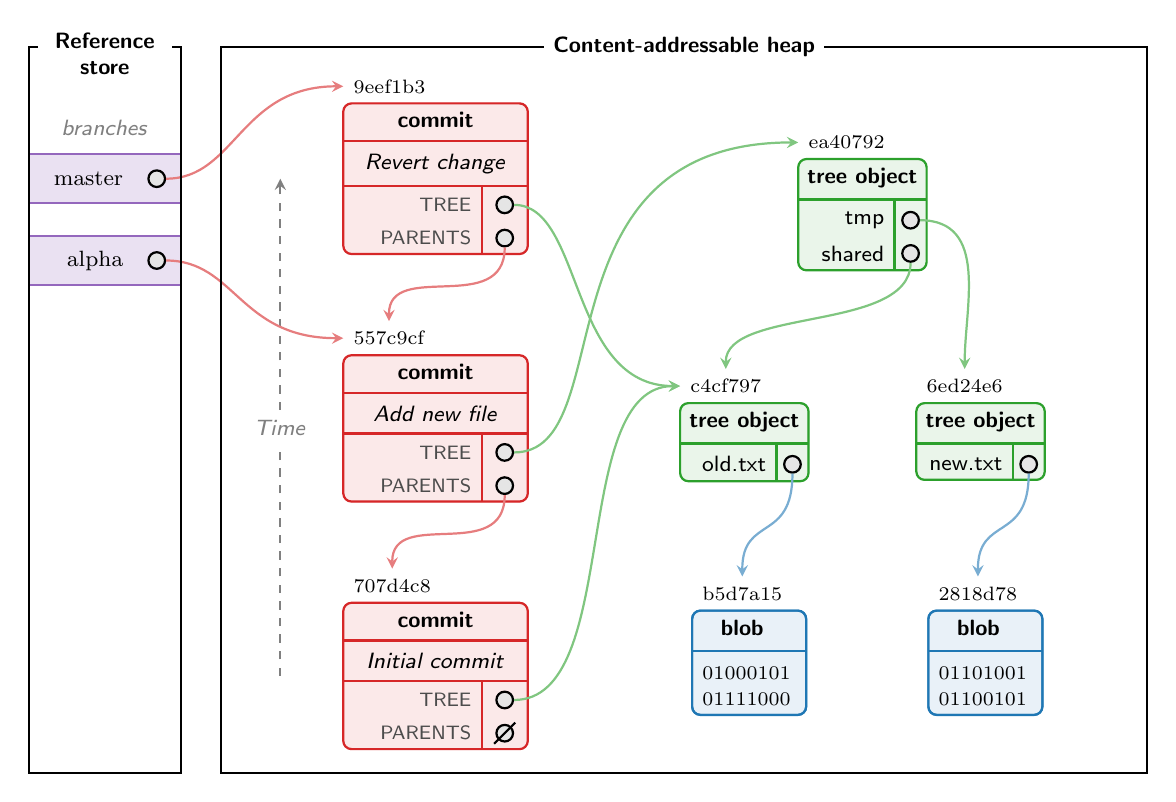
\begin{tikzpicture}[ remember picture , every node/.style={font=\footnotesize\sffamily}
      , hashcirc/.style={draw=black, fill=black!10, circle, inner sep=0pt, minimum size=6pt}
      , hash/.style={font=\scriptsize\ttfamily}
      , commit/.style = {
          , rectangle , rounded corners , inner sep = 0 , fill=TabRed!5 , draw=\blockcolor , line width=0.75pt,
          , minimum width=\commitwidth , minimum height = \commitheight
        }
      , gitptr/.style={draw=TabBlue!60}
      , arrow={->,>=stealth}
    ]

    \def\linespacing{15pt}
    \def\commit[#1]#2(#3)#4(#5)#6(#7) {
      \begin{scope}[local bounding box=#1]
        \begin{scope}[local bounding box=inner-#1]
          \node (#1-init) at (#3) {\textbf{commit}};
          \node[text width = 6em, align=center, below=\linespacing of #1-init.north, anchor=north] (#1-2) {\emph{#5}};
        \end{scope}

        \coordinate (mid) at ($ (#1-init.south)!0.5!(#1-2.north) $);
        \coordinate (triple) at ($ (inner-#1.west |- 0, 0 |- mid)!0.75!(inner-#1.east |- 0, 0 |- mid) $);

        \coordinate[below=0.5*\linespacing of #1-2.south] (x);
        \node[anchor=east, text=black!70] at (triple |- 0, 0 |- x) (#1-tree-label) {\scriptsize TREE};
        \coordinate (x) at ($ (#1-tree-label) + (0, -0.8*\linespacing) $);
        \node[anchor=east, text=black!70] at (triple |- 0, 0 |- x) (#1-parent-label) {\scriptsize PARENTS};
      \end{scope}

      \draw[-, TabRed] (#1.west |- 0, 0 |- mid) -- (#1.east |- 0, 0 |- mid);
      \coordinate (mid) at ($ (#1-2.south)!0.5!(#1-tree-label.north) $);
      \draw[-, TabRed] (#1.west |- 0, 0 |- mid) -- (#1.east |- 0, 0 |- mid);
      \coordinate (triple) at ($ (inner-#1.south west |- 0, 0 |- mid)!0.75!(inner-#1.south east |- 0, 0 |- mid) $);

      \draw[-, TabRed] (triple) -- (triple |- 0, 0 |- #1.south);
      \draw [draw=TabRed, rounded corners=.3em] (#1.north west) rectangle (#1.south east);

      \begin{scope}[on background layer]
        \draw [fill=TabRed!10, draw=TabRed, rounded corners=.3em] (#1.north west) rectangle (#1.south east);
      \end{scope}

      \node[anchor=south west, hash] (#1-hash) at ($ (#1.north west) $) {#7};

      \coordinate (x) at ($ (triple)!0.5!(#1.east) $);
      \node[hashcirc] (#1-tree) at (x |- 0,
      0 |- #1-tree-label) {};

      \node[hashcirc] (#1-parent) at (x |-
      0, 0 |- #1-parent-label) {};
    }

    \def\treecolor{TabGreen}
    \def\tree[#1]#2(#3)#4(#5)#6(#7) {
      \begin{scope}[local bounding box=#1]
        \begin{scope}[local bounding box=inner-#1]
          \node (#1-init) at (#3) {\raisebox{2pt}{\textbf{tree object}}};
        \end{scope}

        \coordinate (mid) at ($ (#1-init) $);
        \coordinate (triple) at ($ (inner-#1.west |- 0, 0 |- mid)!0.75!(inner-#1.east |- 0, 0 |- mid) $);

        \coordinate (x) at ($ (#1-init) + (0, -\linespacing) $);
        \node[anchor=east] at (triple |- 0, 0 |- x) (#1-tree-label) {\footnotesize \textsf{tmp}};
        \coordinate (x) at ($ (#1-tree-label) + (0, -0.8*\linespacing) $);
        \node[anchor=east] at (triple |- 0, 0 |- x) (#1-parent-label) {\footnotesize \textsf{shared}};
      \end{scope}

      \coordinate (mid) at ($ (#1-init)!0.5!(#1-tree-label) $);
      \draw[-, \treecolor] (#1.west |- 0, 0 |- mid) -- (#1.east |- 0, 0 |- mid);
      \coordinate (triple) at ($ (inner-#1.west |- 0, 0 |- mid)!0.75!(inner-#1.east |- 0, 0 |- mid) $);

      \draw[-, \treecolor] (triple) -- (triple |- 0, 0 |- #1.south);
      \draw [draw=\treecolor, rounded corners=.3em] (#1.north west) rectangle (#1.south east);

      \begin{scope}[on background layer]
        \draw [fill=\treecolor!10, draw=\treecolor, rounded corners=.3em] (#1.north west) rectangle (#1.south east);
      \end{scope}

      \node[anchor=south west, hash] (#1-hash) at ($ (#1.north west) $) {#5};

      \coordinate (x) at ($ (triple)!0.5!(#1.east) $);
      \node[hashcirc] (#1-tree) at (x |- 0,
      0 |- #1-tree-label) {};

      \node[hashcirc] (#1-parent) at (x |-
      0, 0 |- #1-parent-label) {};
    }

    \def\treesmall[#1]#2(#3)#4(#5)#6(#7) {
      \begin{scope}[local bounding box=#1]
        \begin{scope}[local bounding box=inner-#1]
          \node (#1-init) at (#3) {\raisebox{2pt}{\textbf{tree object}}};
        \end{scope}

        \coordinate (mid) at ($ (#1-init) $);
        \coordinate (triple) at ($ (inner-#1.west |- 0, 0 |- mid)!0.75!(inner-#1.east |- 0, 0 |- mid) $);

        \coordinate (x) at ($ (#1-init) + (0, -\linespacing) $);
        \node[anchor=east] at (triple |- 0, 0 |- x) (#1-tree-label) {\footnotesize \textsf{#7}};
      \end{scope}

      \coordinate (mid) at ($ (#1-init)!0.5!(#1-tree-label) $);
      \draw[-, \treecolor] (#1.west |- 0, 0 |- mid) -- (#1.east |- 0, 0 |- mid);
      \coordinate (triple) at ($ (inner-#1.west |- 0, 0 |- mid)!0.75!(inner-#1.east |- 0, 0 |- mid) $);

      \draw[-, \treecolor] (triple) -- (triple |- 0, 0 |- #1.south);
      \draw [draw=\treecolor, rounded corners=.3em] (#1.north west) rectangle (#1.south east);

      \begin{scope}[on background layer]
        \draw [fill=\treecolor!10, draw=\treecolor, rounded corners=.3em] (#1.north west) rectangle (#1.south east);
      \end{scope}

      \node[anchor=south west, hash] (#1-hash) at ($ (#1.north west) $) {#5};

      \coordinate (x) at ($ (triple)!0.5!(#1.east) $);
      \node[hashcirc] (#1-tree) at (x |- 0,
      0 |- #1-tree-label) {};
    }

    \def\blobcolor{TabBlue}
    \def\blob[#1]#2(#3)#4(#5)#6(#7) {
      \begin{scope}[local bounding box=#1]
        \begin{scope}[local bounding box=inner-#1]
          \node (#1-init) at (#3) {\ \ \,\textbf{blob}};
        \end{scope}

        \coordinate (triple) at ($ (inner-#1.west |- 0, 0 |- #1-init) $);
        \coordinate (x) at ($ (#1-init) + (0, -0.7*\linespacing) $);
        \node[anchor=north west, text width = 1.2cm] at (triple |- 0, 0 |- x) (#1-tree-label) {\scriptsize\texttt{#7}};
        \coordinate (x) at ($ (#1-tree-label) + (0, -0.8*\linespacing) $);
      \end{scope}

      \coordinate (mid) at ($ (#1-init.south)!0.5!(#1-tree-label.north) $);
      \draw[-, \blobcolor] (#1.west |- 0, 0 |- mid) -- (#1.east |- 0, 0 |- mid);
      \coordinate (triple) at ($ (inner-#1.west |- 0, 0 |- mid)!0.75!(inner-#1.east |- 0, 0 |- mid) $);
      \draw [draw=\blobcolor, rounded corners=.3em] (#1.north west) rectangle (#1.south east);

      \begin{scope}[on background layer]
        \draw [fill=\blobcolor!10, draw=\blobcolor, line width=0.75pt, rounded corners=.3em] (#1.north west) rectangle (#1.south east);
      \end{scope}

      \node[anchor=south west, hash] (#1-hash) at ($ (#1.north west) $) {#5};
    }

    \begin{scope}[local bounding box = heap]
      \begin{scope}[local bounding box = commits]

        \commit[c1] (0, 0) (Revert change) (9eef1b3)

        \coordinate[below = 1.5cm of c1] (commit-2);
        \commit[c2] (commit-2) (Add new file) (557c9cf)

        \coordinate[below = 1.5cm of c2] (commit-3);
        \commit[c3] (commit-3) (Initial commit) (707d4c8)

        \draw[gray, dashed, ->] ($ (c3.west) + (-0.8, 0) $) -- node[midway, fill=white] {\emph{Time}} ($ (c1.west) + (-0.8, 0) $);
      \end{scope}

      \coordinate[right=4.25cm of c1] (tree-1);
      \tree[t1] (tree-1) (ea40792) (
      )

      \coordinate[below left=3.1cm and 1.5cm of tree-1] (tree-2);
      \treesmall[t2] (tree-2) (c4cf797) (old.txt)

      \coordinate[below right=3.1cm and 1.5cm of tree-1] (tree-3);
      \treesmall[t3] (tree-3) (6ed24e6) (new.txt)

      \coordinate[below=2.6cm of tree-2, xshift=-1.5mm] (blob-1);
      \blob[b1] (blob-1) (b5d7a15) (01000101 01111000)

      \coordinate[below=2.6cm of tree-3, xshift=-1.5mm] (blob-2);
      \blob[b2] (blob-2) (2818d78) (01101001 01100101)

      \draw[->, gitptr, draw=TabRed!60] (c1-parent) .. controls ++(0, -1) and ++(0, 1) .. (c2-hash);
      \draw[->, gitptr, draw=TabRed!60] (c2-parent) .. controls ++(0, -1) and ++(0, 1) .. (c3-hash);
      \draw[->, gitptr, draw=TabGreen!60] (c1-tree) .. controls ++(1, 0) and ++(-2, 0) .. (t2-hash);
      \draw[->, gitptr, draw=TabGreen!60] (c2-tree) .. controls ++(1.5, 0) and ++(-4, 0) .. (t1-hash);
      \draw[->, gitptr, draw=TabGreen!60] (c3-tree) .. controls ++(1.5, 0) and ++(-2, 0) .. (t2-hash);

      \draw[->, gitptr, draw=TabGreen!60] (t1-tree) .. controls ++(1, 0) and ++(0, 1) .. (t3-hash);
      \draw[->, gitptr, draw=TabGreen!60] (t1-parent) .. controls ++(0, -1) and ++(0, 1) .. (t2-hash);

      \draw[->, gitptr, draw=TabBlue!60] (t2-tree) .. controls ++(0, -1) and ++(0, 1) .. (b1-hash);
      \draw[->, gitptr, draw=TabBlue!60] (t3-tree) .. controls ++(0, -1) and ++(0, 1) .. (b2-hash);

      \draw [-] ($ (c3-parent.south west) + (-0.05, -0.05) $) -- ($ (c3-parent.north east) + (0.05, 0.05) $);
    \end{scope}

    \begin{scope}[local bounding box=refs]

      \coordinate (t) at (commits.west |- 0, 0 |- c1);

      \node[hashcirc, left = 10mm of t] (r-master-hash) {};
      \node[left = 5pt of r-master-hash, minimum height=1.7em, font=\footnotesize\ttfamily] (r-master) {master};

      \node[hashcirc, below = 0.8cm of r-master-hash] (r-client-hash) {};
      \node[left = 5pt of r-client-hash, minimum height=1.7em, font=\footnotesize\ttfamily] (r-client) {alpha};
    \end{scope}

    \coordinate (ref-mid) at ($ (refs.west)!0.5!(refs.east) $);
    \node[anchor=south,yshift=0.1cm,gray] (branch-label) at (ref-mid |- 0, 0 |- r-master.north) {\emph{branches}};

    \draw[->, gitptr, draw=TabRed!60] (r-master-hash) .. controls ++(1, 0) and ++(-1.9, 0) .. (c1-hash);
    \draw[->, gitptr, draw=TabRed!60] (r-client-hash) .. controls ++(1, 0) and ++(-1.9, 0) .. (c2-hash);

    % Compute outer bounding boxes
    \coordinate (heap-nw) at ($ (heap.north west) + (-\boxspace, \boxspace) $);
    \coordinate (heap-ne) at ($ (heap.north east) + (\boxspace + 1, \boxspace) $);
    \coordinate (heap-sw) at ($ (heap.south west) + (-\boxspace, -\boxspace) $);
    \coordinate (heap-se) at ($ (heap.south east) + (\boxspace + 1, -\boxspace) $);

    \coordinate (divline) at ($(c1.east)!0.5!(t2.west)$);
    \coordinate (labelheight) at ($(heap-se) + (0, -0.5)$);
    \coordinate (causal-label-x) at ($(heap-sw)!0.5!(divline)$);
    \coordinate (merkle-label-x) at ($(heap-se)!0.5!(divline)$);

    \def\refsinnerpad{0.2}

    \coordinate (east-bound) at ($ (refs.east) + (\refsinnerpad, 0) $);
    \coordinate (west-bound) at ($ (refs.west) + (-\refsinnerpad, 0) $);

    \coordinate (refs-nw) at (west-bound |- 0, 0 |- heap-nw);
    \coordinate (refs-ne) at  (east-bound |- 0, 0 |- heap-nw);
    \coordinate (refs-sw) at (west-bound |- 0, 0 |- heap-sw);
    \coordinate (refs-se) at (east-bound |- 0, 0 |- heap-sw);

    \foreach \x in {r-master,r-client} {
        \draw[-, TabPurple] (refs-sw |- 0, 0 |- \x.north) -- (refs-se |- 0, 0 |- \x.north);
        \draw[-, TabPurple] (refs-sw |- 0, 0 |- \x.south) -- (refs-se |- 0, 0 |- \x.south);
        \begin{scope}[on background layer]
          \draw[draw=none, fill=TabPurple!20] (refs-sw |- 0, 0 |- \x.north) rectangle (refs-se |- 0, 0 |-
          \x.south);
        \end{scope}
      }

    \draw[draw, thick] (heap-nw) rectangle (heap-se);
    \draw[draw, thick] (refs-nw) rectangle (refs-se);

    \node[rectangle, fill=white] at ($(heap-nw)!0.5!(heap-ne)$) (heap-label) {\textbf{Content-addressable heap}};

    \node[anchor=north, yshift=5pt, fill=white, text width=1.7cm, outer sep=0, inner sep=0, align=center] at
    ($(refs-nw)!0.5!(refs-ne)$) (refs-label) {\textbf{Reference\\ store}};

  \end{tikzpicture}
\end{figure}


\bigskip
\cref{fig:object-graph} illustrates the state of the reference store and the content-addressable heap of a Git repository after performing the following operations in order: initializing an empty repository; adding a file called \texttt{old.txt} at the root of the repository; creating a commit with the message ``Initial commit''; moving \texttt{old.txt} to a new subfolder called \texttt{shared} and adding a file called \texttt{new.txt} to a new subfolder called \texttt{tmp}; creating a commit with the message ``Add new file''; creating to a new branch called \texttt{alpha}; and finally creating a rollback commit with the message ``Revert change''.

\bigskip
It becomes clear after looking at \cref{fig:object-graph} that the commits, tree nodes and blobs stored in the content-addressable heap form a directed graph \(G = (V, E)\) called the object graph. \(V\) is the set of \emph{graph objects}, defined precisely as:
\begin{align*}
  V & \subset (\{\texttt{`Commit}\} \times H \times \mathcal{P}(H)) \\
    & \ \cup  (\{\texttt{`Node}\} \times \mathcal{P}(S \times H))   \\
    & \ \cup  (\{\texttt{`Blob}\} \times B)
\end{align*}

With \(H = \{0, 1\}^{256}\) the space of 256-bit hash digests, \(S\) the set of valid steps for node paths and \(B\) the set of valid blobs. For every object \(o \in V\), we define \(\texttt{hash}(o) \in H\) as the deterministically-computed address of \(o\). For the sake of clarity, we also define helper functions to be used in pseudo-code algorithms. for a commit \(c = (\texttt{`Commit}, t, ps) \in V\), let \(\texttt{tree}(c) := t\) be the address of the root node for \(c\), and let \(\texttt{parents}(c) := ps\) be the set of addresses of the parent commits of \(c\). For a node \(n = (\texttt{`Node}, ch) \in V\), let \(\texttt{children}(n) := ch\) be the set of \((step, hash) \in P \times S\) pairs for every child node of \(n\). For a blob \(b = (\texttt{`Blob}, c) \in V\), let \(\texttt{content}(b) := c\) be the content of \(b\).

Finally, for any object \(o \in V\) in the graph, we define the successors of \(o\) as:

\begin{equation*}
  successors(o) =
  \begin{cases}
    \{\texttt{tree}(o)\} \cup \texttt{parents}(o)         & \text{if $o$ is a commit}
    \\
    \{hash \ | \ (step, hash) \in \texttt{children}(o) \} & \text{if $o$ is a node}
    \\
    \emptyset                                             & \text{if $o$ is a blob}
  \end{cases}
\end{equation*}

\bigskip
Since the address of every object in the graph derived from the address of its parents, it should be clear that the object graph is acyclic--assuming that the hash function is reasonably collision-resistant. Formally speaking, this data structure is called a \emph{Merkle DAG}--a generalization of \emph{Merkle trees} which were first introduced in~\cite{merkle88} to compute cryptographic signatures.

\subsection{The Irmin database library}

\emph{Irmin}~\cite{irmin} is an open-source distributed
database library written in OCaml, which is maintained by Tarides~\cite{tarides} as part of the MirageOS~\cite{mirage}~\cite{mirage-paper} project. It allows developers to build branchable, mergeable distributed data stores; and supports--among other things--snapshotting, custom storage layers and custom datatypes. Introductory research material for Irmin can be found at \cite{irmin15} and \cite{irmin19}.

Irmin was initially built as an extension of Xenstore~\cite{xenstore}, and has since been used as a backend for many OCaml applications, both within the MirageOS ecosystem--for instance in \texttt{mirage/arp}~\cite{mirage-arp}, \texttt{mirage/ocaml-dns}~\cite{mirage-dns} or \texttt{roburio/caldav}~\cite{roburio-caldav}--and outside of it, for instance in \emph{continuous integration} systems which build thousands of artefacts daily; or in the \emph{Docker for Desktop} client.

Notably, Irmin serves as the storage backend for nodes of the Tezos~\cite{tezos} blockchain, which was first described in~\cite{tezos14}. At the time of writing, this requires supporting the storage of roughly 350 million objects--for a total disk footprint of 37 GB. \emph{Up-to-date figures can be computed using the script at~\cite{tree-statistics}.}

Practically, an Irmin database is created by supplying several modules to the \texttt{Irmin.Make} functor: the function used to hash objects; the storage backend; and the datatype of branch handles, node labels and blobs. Using the database is then akin to manipulating a Git repository: as illustrated in \cref{lst:irmin-example}, the user can initialize the database; checkout a branch; store one or many versioned values in the branch by creating a commit; etc. Since most operations result in the creation of a new commit, changes in an Irmin database are always non-destructive and can be rolled back safely if necessary. Similarly to Git, Irmin also provides an API to synchronize with remote databases using \texttt{push} and \texttt{pull} operations--although the specifics are out of the scope of this internship. \cref{app:irmin-interface} contains the full database interface for reference.

\begin{figure}[ht]
  \caption{A few basic operations on an Irmin database.}
  \label{lst:irmin-example}

  \centering
  \vspace{-1em}
  \begin{minted}{ocaml}
(* The return values of most operations are wrapped inside the [Lwt.t]
   concurrency monad, so we unwrap them using the OCaml monadic syntax. *)
let (let*) = Lwt.bind

(* Create a new Irmin database with SHA256 hashes, in-memory storage,
   string branches, string paths and floating-point blobs. *)
module Database = Make (Hash.SHA256) (Backend.Memory)
                       (Types.String) (Types.String) (Types.Float)

(* Create the database by forwarding options to the backend. *)
let* t = Database.create () in

(* Checkout the master branch. *)
let* master = Database.checkout t "master" in

(* Commit a first value under path /foo. *)
let* c1 = Database.set ~message:"First commit." master ["foo"] 0.0 in

(* Create a new `checkpoint` branch pointing to the first commit. *)
let* () = Database.Branches.set t "checkpoint" c1 in

(* Commit multiple values at once under paths /bar/baz and /bar/boz. *)
let* c2 = Database.set_tree ~message:"Second commit." master ["bar"]
            (`Node [("baz", `Blob 1.0); ("boz", `Blob 2.0)]) in

(* Retrieve the value of at /bar/baz from the `master` branch.
   Note that this value wouldn't exist in the `checkpoint` branch. *)
let* v = Database.get master ["bar"; "baz"] in assert (v = 0.0)
    \end{minted}
\end{figure}


Note that, unless otherwise mentioned, all the code listings in this thesis are excerpts from the \texttt{irmin-toy}~\cite{irmin-toy-github} library instead of \texttt{irmin}~\cite{irmin-github}. It is a simplified model which I implemented from scratch during this internship, and which focuses only on the parts of Irmin that are relevant to my work.

\bigskip
One of the key aspects of Irmin is \emph{modularity}: as highlighted at the beginning of \cref{lst:irmin-example}, the hash function, storage backend and object datatypes can be swapped for any other module--either provided by Irmin or user-defined--with the right signature. Irmin comes with a few storage backends out of the box: \texttt{irmin-mem}, which stores objects in a hashtable in memory; \texttt{irmin-fs}, which persists serialized objects on a POSIX filesystem; \texttt{irmin-git}, which provides a layer of compatibility with Git repositories; and \texttt{irmin-pack}, which persists serialized objects in a single large file similar to a block device. Storage backends must satisfy the interface from lines 398 to 581 of \cref{app:irmin-interface}: in short, they must provide both an \texttt{ATOMIC\_WRITE\_STORE} and a \texttt{CONTENT\_ADDRESSABLE\_STORE} implementation; the \texttt{ATOMIC\_WRITE\_STORE} is a mutable store which will provide a way to atomically read, update and remove branch pointers; and the \texttt{CONTENT\_ADDRESSABLE\_STORE} is an immutable store which will provide a way to store and fetch objects addressed by a deterministic hash--here commits, tree nodes and blobs.

\bigskip
This is strongly reminiscent of the internals of Git--with the \texttt{ATOMIC\_WRITE\_STORE} acting as the Git reference store and the several \texttt{CONTENT\_ADDRESSABLE\_STORE} together forming the Git content-addressable heap. For this reason, we will extend the notion of object graph defined above to Irmin backends and the objects that they store.

\subsection{Garbage collection}

Generally speaking, \emph{garbage collection} designates the techniques which automatically reclaim the memory occupied by objects which are no longer in use by a program. This alleviates the burden of manual memory management from the programmer, making it easier to write programs while also eliminating a large class of bugs--for instance \emph{dangling pointer} and \emph{double free} bugs.

While the term \emph{garbage collection} is mostly used in the context of memory-managed programming languages, it can also be generalized to designate any system which automatically reclaims unused memory. In particular, the Git version control system is designed in such a way that aborting some operations or rolling back changes can leave unused objects in the database. To alleviate this issue, Git uses garbage collection to periodically find unused objects in the content-addressable heap and remove them from the disk--the garbage collector can also be explicitly called using \texttt{git\ gc}~\cite{git-gc}.

Since Irmin shares its internal representation with Git, it also suffers from the same issue. To better illustrate the situation, let's look back at the database from \cref{fig:object-graph}. If we removed the \texttt{alpha} branch by calling \mintinline{ocaml}{Database.Branches.remove t "alpha"}, and subsequently rolled back the \texttt{master} branch to the initial commit by calling \mintinline{ocaml}{Database.Branches.set t "master" commit_707d4c8}, we would be left with the database from \cref{fig:object-graph-gc}--which contains two unused commits, two unused nodes, and an unused blob. Since these five objects can no longer be reached by the user, they could safely be removed from the database to free up disk space.

\begin{figure}[ht]
  \caption{Object graph of a Git repository after removing \texttt{alpha} and rolling back \texttt{master}.\\ \textit{(Less opaque elements are no longer reachable from any branch.)}}
  \label{fig:object-graph-gc}

  \centering
  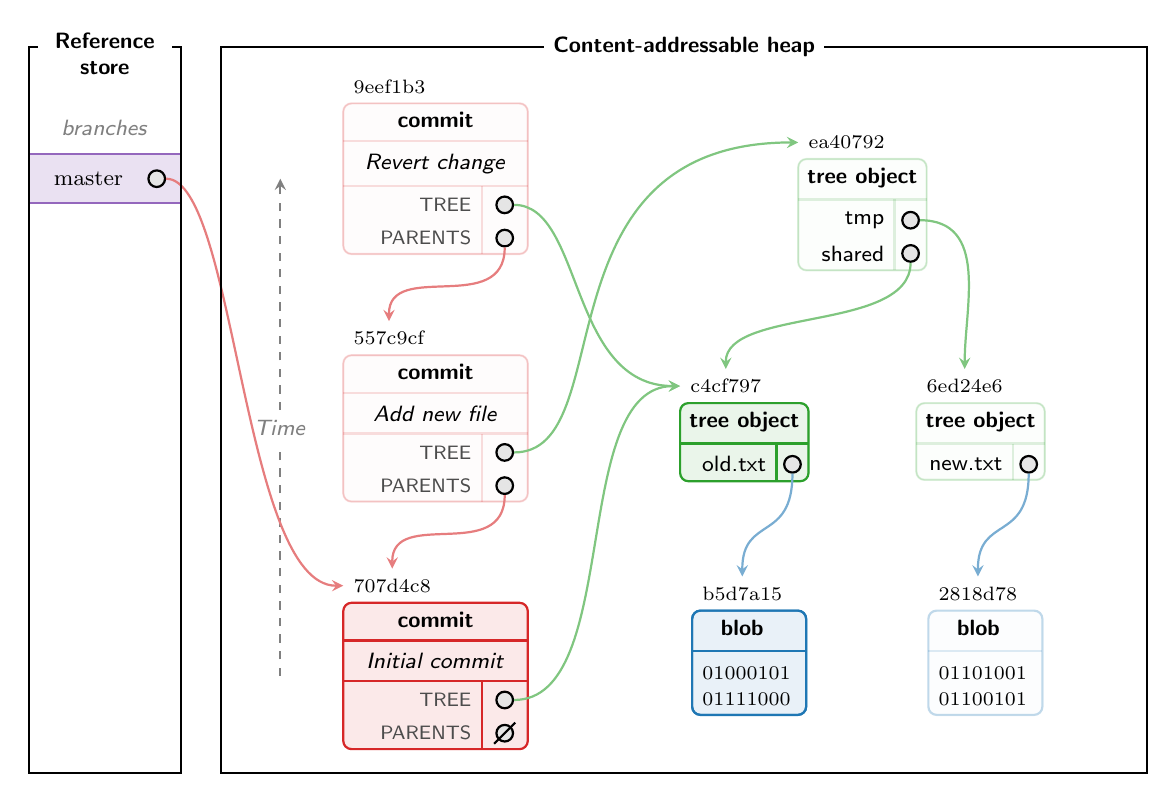
\begin{tikzpicture}[ remember picture , every node/.style={font=\footnotesize\sffamily}
      , hashcirc/.style={draw=black, fill=black!10, circle, inner sep=0pt, minimum size=6pt}
      , hash/.style={font=\scriptsize\ttfamily}
      , commit/.style = {
          , rectangle , rounded corners , inner sep = 0 , fill=TabRed!5 , draw=\blockcolor , line width=0.75pt,
          , minimum width=\commitwidth , minimum height = \commitheight
        }
      , gitptr/.style={draw=TabBlue!60}
      , arrow={->,>=stealth}
    ]

    \def\linespacing{15pt}
    \def\commit[#1]#2(#3)#4(#5)#6(#7) {
      \begin{scope}[local bounding box=#1]
        \begin{scope}[local bounding box=inner-#1]
          \node (#1-init) at (#3) {\textbf{commit}};
          \node[text width = 6em, align=center, below=\linespacing of #1-init.north, anchor=north] (#1-2) {\emph{#5}};
        \end{scope}

        \coordinate (mid) at ($ (#1-init.south)!0.5!(#1-2.north) $);
        \coordinate (triple) at ($ (inner-#1.west |- 0, 0 |- mid)!0.75!(inner-#1.east |- 0, 0 |- mid) $);

        \coordinate[below=0.5*\linespacing of #1-2.south] (x);
        \node[anchor=east, text=black!70] at (triple |- 0, 0 |- x) (#1-tree-label) {\scriptsize TREE};
        \coordinate (x) at ($ (#1-tree-label) + (0, -0.8*\linespacing) $);
        \node[anchor=east, text=black!70] at (triple |- 0, 0 |- x) (#1-parent-label) {\scriptsize PARENTS};
      \end{scope}

      \draw[-, TabRed] (#1.west |- 0, 0 |- mid) -- (#1.east |- 0, 0 |- mid);
      \coordinate (mid) at ($ (#1-2.south)!0.5!(#1-tree-label.north) $);
      \draw[-, TabRed] (#1.west |- 0, 0 |- mid) -- (#1.east |- 0, 0 |- mid);
      \coordinate (triple) at ($ (inner-#1.south west |- 0, 0 |- mid)!0.75!(inner-#1.south east |- 0, 0 |- mid) $);

      \draw[-, TabRed] (triple) -- (triple |- 0, 0 |- #1.south);
      \draw [draw=TabRed, rounded corners=.3em] (#1.north west) rectangle (#1.south east);

      \begin{scope}[on background layer]
        \draw [fill=TabRed!10, draw=TabRed, rounded corners=.3em] (#1.north west) rectangle (#1.south east);
      \end{scope}

      \node[anchor=south west, hash] (#1-hash) at ($ (#1.north west) $) {#7};

      \coordinate (x) at ($ (triple)!0.5!(#1.east) $);
      \node[hashcirc] (#1-tree) at (x |- 0,
      0 |- #1-tree-label) {};

      \node[hashcirc] (#1-parent) at (x |-
      0, 0 |- #1-parent-label) {};
    }
    \def\deadcommit[#1]#2(#3)#4(#5)#6(#7) {
      \begin{scope}[local bounding box=#1]
        \begin{scope}[local bounding box=inner-#1]
          \node (#1-init) at (#3) {\textbf{commit}};
          \node[text width = 6em, align=center, below=\linespacing of #1-init.north, anchor=north] (#1-2) {\emph{#5}};
        \end{scope}

        \coordinate (mid) at ($ (#1-init.south)!0.5!(#1-2.north) $);
        \coordinate (triple) at ($ (inner-#1.west |- 0, 0 |- mid)!0.75!(inner-#1.east |- 0, 0 |- mid) $);

        \coordinate[below=0.5*\linespacing of #1-2.south] (x);
        \node[anchor=east, text=black!70] at (triple |- 0, 0 |- x) (#1-tree-label) {\scriptsize TREE};
        \coordinate (x) at ($ (#1-tree-label) + (0, -0.8*\linespacing) $);
        \node[anchor=east, text=black!70] at (triple |- 0, 0 |- x) (#1-parent-label) {\scriptsize PARENTS};
      \end{scope}

      \draw[-, TabRed, opacity=.15] (#1.west |- 0, 0 |- mid) -- (#1.east |- 0, 0 |- mid);
      \coordinate (mid) at ($ (#1-2.south)!0.5!(#1-tree-label.north) $);
      \draw[-, TabRed, opacity=.15] (#1.west |- 0, 0 |- mid) -- (#1.east |- 0, 0 |- mid);
      \coordinate (triple) at ($ (inner-#1.south west |- 0, 0 |- mid)!0.75!(inner-#1.south east |- 0, 0 |- mid) $);

      \draw[-, TabRed, opacity=.15] (triple) -- (triple |- 0, 0 |- #1.south);
      \draw [draw=TabRed, opacity=.15, rounded corners=.3em] (#1.north west) rectangle (#1.south east);

      \begin{scope}[on background layer]
        \draw [fill=TabRed!10, draw=TabRed, rounded corners=.3em, opacity=.15] (#1.north west) rectangle (#1.south east);
      \end{scope}

      \node[anchor=south west, hash] (#1-hash) at ($ (#1.north west) $) {#7};

      \coordinate (x) at ($ (triple)!0.5!(#1.east) $);
      \node[hashcirc] (#1-tree) at (x |- 0,
      0 |- #1-tree-label) {};

      \node[hashcirc] (#1-parent) at (x |-
      0, 0 |- #1-parent-label) {};
    }

    \def\treecolor{TabGreen}
    \def\tree[#1]#2(#3)#4(#5)#6(#7) {
      \begin{scope}[local bounding box=#1]
        \begin{scope}[local bounding box=inner-#1]
          \node (#1-init) at (#3) {\raisebox{2pt}{\textbf{tree object}}};
        \end{scope}

        \coordinate (mid) at ($ (#1-init) $);
        \coordinate (triple) at ($ (inner-#1.west |- 0, 0 |- mid)!0.75!(inner-#1.east |- 0, 0 |- mid) $);

        \coordinate (x) at ($ (#1-init) + (0, -\linespacing) $);
        \node[anchor=east] at (triple |- 0, 0 |- x) (#1-tree-label) {\footnotesize \textsf{tmp}};
        \coordinate (x) at ($ (#1-tree-label) + (0, -0.8*\linespacing) $);
        \node[anchor=east] at (triple |- 0, 0 |- x) (#1-parent-label) {\footnotesize \textsf{shared}};
      \end{scope}

      \coordinate (mid) at ($ (#1-init)!0.5!(#1-tree-label) $);
      \draw[-, \treecolor] (#1.west |- 0, 0 |- mid) -- (#1.east |- 0, 0 |- mid);
      \coordinate (triple) at ($ (inner-#1.west |- 0, 0 |- mid)!0.75!(inner-#1.east |- 0, 0 |- mid) $);

      \draw[-, \treecolor] (triple) -- (triple |- 0, 0 |- #1.south);
      \draw [draw=\treecolor, rounded corners=.3em] (#1.north west) rectangle (#1.south east);

      \begin{scope}[on background layer]
        \draw [fill=\treecolor!10, draw=\treecolor, rounded corners=.3em] (#1.north west) rectangle (#1.south east);
      \end{scope}

      \node[anchor=south west, hash] (#1-hash) at ($ (#1.north west) $) {#5};

      \coordinate (x) at ($ (triple)!0.5!(#1.east) $);
      \node[hashcirc] (#1-tree) at (x |- 0,
      0 |- #1-tree-label) {};

      \node[hashcirc] (#1-parent) at (x |-
      0, 0 |- #1-parent-label) {};
    }
    \def\deadtree[#1]#2(#3)#4(#5)#6(#7) {
      \begin{scope}[local bounding box=#1]
        \begin{scope}[local bounding box=inner-#1]
          \node (#1-init) at (#3) {\raisebox{2pt}{\textbf{tree object}}};
        \end{scope}

        \coordinate (mid) at ($ (#1-init) $);
        \coordinate (triple) at ($ (inner-#1.west |- 0, 0 |- mid)!0.75!(inner-#1.east |- 0, 0 |- mid) $);

        \coordinate (x) at ($ (#1-init) + (0, -\linespacing) $);
        \node[anchor=east] at (triple |- 0, 0 |- x) (#1-tree-label) {\footnotesize \textsf{tmp}};
        \coordinate (x) at ($ (#1-tree-label) + (0, -0.8*\linespacing) $);
        \node[anchor=east] at (triple |- 0, 0 |- x) (#1-parent-label) {\footnotesize \textsf{shared}};
      \end{scope}

      \coordinate (mid) at ($ (#1-init)!0.5!(#1-tree-label) $);
      \draw[-, \treecolor, opacity=.15] (#1.west |- 0, 0 |- mid) -- (#1.east |- 0, 0 |- mid);
      \coordinate (triple) at ($ (inner-#1.west |- 0, 0 |- mid)!0.75!(inner-#1.east |- 0, 0 |- mid) $);

      \draw[-, \treecolor, opacity=.15] (triple) -- (triple |- 0, 0 |- #1.south);
      \draw [draw=\treecolor, opacity=.15, rounded corners=.3em] (#1.north west) rectangle (#1.south east);

      \begin{scope}[on background layer]
        \draw [fill=\treecolor!10, draw=\treecolor, opacity=.15, rounded corners=.3em] (#1.north west) rectangle (#1.south east);
      \end{scope}

      \node[anchor=south west, hash] (#1-hash) at ($ (#1.north west) $) {#5};

      \coordinate (x) at ($ (triple)!0.5!(#1.east) $);
      \node[hashcirc] (#1-tree) at (x |- 0,
      0 |- #1-tree-label) {};

      \node[hashcirc] (#1-parent) at (x |-
      0, 0 |- #1-parent-label) {};
    }

    \def\treesmall[#1]#2(#3)#4(#5)#6(#7) {
      \begin{scope}[local bounding box=#1]
        \begin{scope}[local bounding box=inner-#1]
          \node (#1-init) at (#3) {\raisebox{2pt}{\textbf{tree object}}};
        \end{scope}

        \coordinate (mid) at ($ (#1-init) $);
        \coordinate (triple) at ($ (inner-#1.west |- 0, 0 |- mid)!0.75!(inner-#1.east |- 0, 0 |- mid) $);

        \coordinate (x) at ($ (#1-init) + (0, -\linespacing) $);
        \node[anchor=east] at (triple |- 0, 0 |- x) (#1-tree-label) {\footnotesize \textsf{#7}};
      \end{scope}

      \coordinate (mid) at ($ (#1-init)!0.5!(#1-tree-label) $);
      \draw[-, \treecolor] (#1.west |- 0, 0 |- mid) -- (#1.east |- 0, 0 |- mid);
      \coordinate (triple) at ($ (inner-#1.west |- 0, 0 |- mid)!0.75!(inner-#1.east |- 0, 0 |- mid) $);

      \draw[-, \treecolor] (triple) -- (triple |- 0, 0 |- #1.south);
      \draw [draw=\treecolor, rounded corners=.3em] (#1.north west) rectangle (#1.south east);

      \begin{scope}[on background layer]
        \draw [fill=\treecolor!10, draw=\treecolor, rounded corners=.3em] (#1.north west) rectangle (#1.south east);
      \end{scope}

      \node[anchor=south west, hash] (#1-hash) at ($ (#1.north west) $) {#5};

      \coordinate (x) at ($ (triple)!0.5!(#1.east) $);
      \node[hashcirc] (#1-tree) at (x |- 0,
      0 |- #1-tree-label) {};
    }
    \def\deadtreesmall[#1]#2(#3)#4(#5)#6(#7) {
      \begin{scope}[local bounding box=#1]
        \begin{scope}[local bounding box=inner-#1]
          \node (#1-init) at (#3) {\raisebox{2pt}{\textbf{tree object}}};
        \end{scope}

        \coordinate (mid) at ($ (#1-init) $);
        \coordinate (triple) at ($ (inner-#1.west |- 0, 0 |- mid)!0.75!(inner-#1.east |- 0, 0 |- mid) $);

        \coordinate (x) at ($ (#1-init) + (0, -\linespacing) $);
        \node[anchor=east] at (triple |- 0, 0 |- x) (#1-tree-label) {\footnotesize \textsf{#7}};
      \end{scope}

      \coordinate (mid) at ($ (#1-init)!0.5!(#1-tree-label) $);
      \draw[-, \treecolor, opacity=.15] (#1.west |- 0, 0 |- mid) -- (#1.east |- 0, 0 |- mid);
      \coordinate (triple) at ($ (inner-#1.west |- 0, 0 |- mid)!0.75!(inner-#1.east |- 0, 0 |- mid) $);

      \draw[-, \treecolor, opacity=.15] (triple) -- (triple |- 0, 0 |- #1.south);
      \draw [draw=\treecolor, opacity=.15, rounded corners=.3em] (#1.north west) rectangle (#1.south east);

      \begin{scope}[on background layer]
        \draw [fill=\treecolor!10, draw=\treecolor, opacity=.15, rounded corners=.3em] (#1.north west) rectangle (#1.south east);
      \end{scope}

      \node[anchor=south west, hash] (#1-hash) at ($ (#1.north west) $) {#5};

      \coordinate (x) at ($ (triple)!0.5!(#1.east) $);
      \node[hashcirc] (#1-tree) at (x |- 0,
      0 |- #1-tree-label) {};
    }

    \def\blobcolor{TabBlue}
    \def\blob[#1]#2(#3)#4(#5)#6(#7) {
      \begin{scope}[local bounding box=#1]
        \begin{scope}[local bounding box=inner-#1]
          \node (#1-init) at (#3) {\ \ \,\textbf{blob}};
        \end{scope}

        \coordinate (triple) at ($ (inner-#1.west |- 0, 0 |- #1-init) $);
        \coordinate (x) at ($ (#1-init) + (0, -0.7*\linespacing) $);
        \node[anchor=north west, text width = 1.2cm] at (triple |- 0, 0 |- x) (#1-tree-label) {\scriptsize\texttt{#7}};
        \coordinate (x) at ($ (#1-tree-label) + (0, -0.8*\linespacing) $);
      \end{scope}

      \coordinate (mid) at ($ (#1-init.south)!0.5!(#1-tree-label.north) $);
      \draw[-, \blobcolor] (#1.west |- 0, 0 |- mid) -- (#1.east |- 0, 0 |- mid);
      \coordinate (triple) at ($ (inner-#1.west |- 0, 0 |- mid)!0.75!(inner-#1.east |- 0, 0 |- mid) $);
      \draw [draw=\blobcolor, rounded corners=.3em] (#1.north west) rectangle (#1.south east);

      \begin{scope}[on background layer]
        \draw [fill=\blobcolor!10, draw=\blobcolor, line width=0.75pt, rounded corners=.3em] (#1.north west) rectangle (#1.south east);
      \end{scope}

      \node[anchor=south west, hash] (#1-hash) at ($ (#1.north west) $) {#5};
    }
    \def\deadblob[#1]#2(#3)#4(#5)#6(#7) {
      \begin{scope}[local bounding box=#1]
        \begin{scope}[local bounding box=inner-#1]
          \node (#1-init) at (#3) {\ \ \,\textbf{blob}};
        \end{scope}

        \coordinate (triple) at ($ (inner-#1.west |- 0, 0 |- #1-init) $);
        \coordinate (x) at ($ (#1-init) + (0, -0.7*\linespacing) $);
        \node[anchor=north west, text width = 1.2cm] at (triple |- 0, 0 |- x) (#1-tree-label) {\scriptsize\texttt{#7}};
        \coordinate (x) at ($ (#1-tree-label) + (0, -0.8*\linespacing) $);
      \end{scope}

      \coordinate (mid) at ($ (#1-init.south)!0.5!(#1-tree-label.north) $);
      \draw[-, \blobcolor, opacity=.15] (#1.west |- 0, 0 |- mid) -- (#1.east |- 0, 0 |- mid);
      \coordinate (triple) at ($ (inner-#1.west |- 0, 0 |- mid)!0.75!(inner-#1.east |- 0, 0 |- mid) $);
      \draw [draw=\blobcolor, opacity=.15, rounded corners=.3em] (#1.north west) rectangle (#1.south east);

      \begin{scope}[on background layer]
        \draw [fill=\blobcolor!10, draw=\blobcolor, opacity=.15, line width=0.75pt, rounded corners=.3em] (#1.north west) rectangle (#1.south east);
      \end{scope}

      \node[anchor=south west, hash] (#1-hash) at ($ (#1.north west) $) {#5};
    }

    \begin{scope}[local bounding box = heap]
      \begin{scope}[local bounding box = commits]

        \deadcommit[c1] (0, 0) (Revert change) (9eef1b3)

        \coordinate[below = 1.5cm of c1] (commit-2);
        \deadcommit[c2] (commit-2) (Add new file) (557c9cf)

        \coordinate[below = 1.5cm of c2] (commit-3);
        \commit[c3] (commit-3) (Initial commit) (707d4c8)

        \draw[gray, dashed, ->] ($ (c3.west) + (-0.8, 0) $) -- node[midway, fill=white] {\emph{Time}} ($ (c1.west) + (-0.8, 0) $);
      \end{scope}

      \coordinate[right=4.25cm of c1] (tree-1);
      \deadtree[t1] (tree-1) (ea40792) (
      )

      \coordinate[below left=3.1cm and 1.5cm of tree-1] (tree-2);
      \treesmall[t2] (tree-2) (c4cf797) (old.txt)

      \coordinate[below right=3.1cm and 1.5cm of tree-1] (tree-3);
      \deadtreesmall[t3] (tree-3) (6ed24e6) (new.txt)

      \coordinate[below=2.6cm of tree-2, xshift=-1.5mm] (blob-1);
      \blob[b1] (blob-1) (b5d7a15) (01000101 01111000)

      \coordinate[below=2.6cm of tree-3, xshift=-1.5mm] (blob-2);
      \deadblob[b2] (blob-2) (2818d78) (01101001 01100101)

      \draw[->, gitptr, draw=TabRed!60] (c1-parent) .. controls ++(0, -1) and ++(0, 1) .. (c2-hash);
      \draw[->, gitptr, draw=TabRed!60] (c2-parent) .. controls ++(0, -1) and ++(0, 1) .. (c3-hash);
      \draw[->, gitptr, draw=TabGreen!60] (c1-tree) .. controls ++(1, 0) and ++(-2, 0) .. (t2-hash);
      \draw[->, gitptr, draw=TabGreen!60] (c2-tree) .. controls ++(1.5, 0) and ++(-4, 0) .. (t1-hash);
      \draw[->, gitptr, draw=TabGreen!60] (c3-tree) .. controls ++(1.5, 0) and ++(-2, 0) .. (t2-hash);

      \draw[->, gitptr, draw=TabGreen!60] (t1-tree) .. controls ++(1, 0) and ++(0, 1) .. (t3-hash);
      \draw[->, gitptr, draw=TabGreen!60] (t1-parent) .. controls ++(0, -1) and ++(0, 1) .. (t2-hash);

      \draw[->, gitptr, draw=TabBlue!60] (t2-tree) .. controls ++(0, -1) and ++(0, 1) .. (b1-hash);
      \draw[->, gitptr, draw=TabBlue!60] (t3-tree) .. controls ++(0, -1) and ++(0, 1) .. (b2-hash);

      \draw [-] ($ (c3-parent.south west) + (-0.05, -0.05) $) -- ($ (c3-parent.north east) + (0.05, 0.05) $);
    \end{scope}

    \begin{scope}[local bounding box=refs]

      \coordinate (t) at (commits.west |- 0, 0 |- c1);

      \node[hashcirc, left = 10mm of t] (r-master-hash) {};
      \node[left = 5pt of r-master-hash, minimum height=1.7em, font=\footnotesize\ttfamily] (r-master) {master};
    \end{scope}

    \coordinate (ref-mid) at ($ (refs.west)!0.5!(refs.east) $);
    \node[anchor=south,yshift=0.1cm,gray] (branch-label) at (ref-mid |- 0, 0 |- r-master.north) {\emph{branches}};

    \draw[->, gitptr, draw=TabRed!60] (r-master-hash) .. controls ++(1, 0) and ++(-1.9, 0) .. (c3-hash);

    % Compute outer bounding boxes
    \coordinate (heap-nw) at ($ (heap.north west) + (-\boxspace, \boxspace) $);
    \coordinate (heap-ne) at ($ (heap.north east) + (\boxspace + 1, \boxspace) $);
    \coordinate (heap-sw) at ($ (heap.south west) + (-\boxspace, -\boxspace) $);
    \coordinate (heap-se) at ($ (heap.south east) + (\boxspace + 1, -\boxspace) $);

    \coordinate (divline) at ($(c1.east)!0.5!(t2.west)$);
    \coordinate (labelheight) at ($(heap-se) + (0, -0.5)$);
    \coordinate (causal-label-x) at ($(heap-sw)!0.5!(divline)$);
    \coordinate (merkle-label-x) at ($(heap-se)!0.5!(divline)$);

    \def\refsinnerpad{0.2}

    \coordinate (east-bound) at ($ (refs.east) + (\refsinnerpad, 0) $);
    \coordinate (west-bound) at ($ (refs.west) + (-\refsinnerpad, 0) $);

    \coordinate (refs-nw) at (west-bound |- 0, 0 |- heap-nw);
    \coordinate (refs-ne) at  (east-bound |- 0, 0 |- heap-nw);
    \coordinate (refs-sw) at (west-bound |- 0, 0 |- heap-sw);
    \coordinate (refs-se) at (east-bound |- 0, 0 |- heap-sw);

    \foreach \x in {r-master} {
        \draw[-, TabPurple] (refs-sw |- 0, 0 |- \x.north) -- (refs-se |- 0, 0 |- \x.north);
        \draw[-, TabPurple] (refs-sw |- 0, 0 |- \x.south) -- (refs-se |- 0, 0 |- \x.south);
        \begin{scope}[on background layer]
          \draw[draw=none, fill=TabPurple!20] (refs-sw |- 0, 0 |- \x.north) rectangle (refs-se |- 0, 0 |-
          \x.south);
        \end{scope}
      }

    \draw[draw, thick] (heap-nw) rectangle (heap-se);
    \draw[draw, thick] (refs-nw) rectangle (refs-se);

    \node[rectangle, fill=white] at ($(heap-nw)!0.5!(heap-ne)$) (heap-label) {\textbf{Content-addressable heap}};

    \node[anchor=north, yshift=5pt, fill=white, text width=1.7cm, outer sep=0, inner sep=0, align=center] at
    ($(refs-nw)!0.5!(refs-ne)$) (refs-label) {\textbf{Reference\\ store}};

  \end{tikzpicture}
  \vspace{1em}
\end{figure}


\bigskip
This brings us to the purpose of this internship: \emph{to design and implement a garbage collection scheme for Irmin}. With the context above in mind, this can be reformulated into the following: \emph{to design and implement a scheme which identifies unreachable objects in an Irmin object graph and removes them from their respective \texttt{CONTENT\_ADDRESSABLE\_STORE} to free up space.}

\bigskip
There were several constraints to take into account while designing this scheme--some of which are common to most garbage collection schemes~\cite{handbook}, while others are tied to the scale and performance requirements of Irmin, especially in the Tezos use case.

\begin{itemize}
  \item \emph{Safety.}
        Most importantly, any garbage collection scheme should be \emph{safe}, meaning that the collector must never reclaim objects of the graph which are still accessible, or could become accessible later.

  \item \emph{Completeness and promptness.}
        Any garbage collection scheme should ideally be \emph{complete}, meaning that all garbage--unreachable objects--should be reclaimed. Note that it might not always be possible to reclaim all garbage at the end of every \emph{collection cycle}--see the section on \emph{Concurrent garbage collection} for details. Instead, some objects may become \emph{floating garbage}, meaning that they will only be reclaimed during a later cycle. This prompts an alternate definition of \emph{completeness} as the \emph{eventual} reclamation of all unreachable objects; and the introduction of \emph{promptness}: the number of \emph{collection cycles} required before an unreachable object can be reclaimed.

  \item \emph{Low pause times.}
        Most garbage collection schemes require the rest of the application to stop partially or entirely during a \emph{collection cycle}. While this requirement can be alleviated with \emph{concurrent garbage collection} techniques, it is generally impossible to avoid pauses entirely. Instead, a garbage collection scheme should try to stop the rest of the application for as little time as possible--although this usually requires a trade-off with promptness, throughput or memory overhead. This constraint was particularly significant during this internship, because some applications built using Irmin are particularly latency-critical--e.g.~Tezos nodes.

  \item \emph{Low memory overhead.}
        During a collection cycle, garbage collectors should use as little additional memory as possible. This was also a significant constraint during this internship, notably because the total memory usage of Irmin inside Tezos nodes is capped at a few hundred megabytes.

  \item \emph{Low storage overhead.}
        Collection scheme targeting Irmin should avoid storing additional data alongside objects--usually on disk--solely for the purpose of facilitating garbage collection. The reasoning behind this constraint is that some applications built using Irmin might not require the garbage collection feature, so we should not penalize them indirectly by increasing the disk usage of Irmin.

  \item \emph{Modularity.}
        Finally, since one of the key aspects of Irmin is modularity--see above for more details--the garbage collection scheme should be designed around the same idea. Practically, this means that garbage collection should work regardless of the particular storage backend used--whether in memory, on disk or in a pack-file--while accommodating for the specific trade-offs of each backend.
\end{itemize}

\newpage

\section{Garbage collection strategies}

While the idea of--and the challenges associated with--garbage collection in the context of Irmin differ slightly from what is usually found in literature, my general approach during this internship was to start by looking there for ideas and algorithms, and then try to adapt them to our problem where relevant. Note that this approach was not always successful, notably because some usual assumptions about garbage collection might not apply to objects stored on Irmin backends which are orders of magnitude slower than RAM--e.g.~\texttt{irmin-fs} or \texttt{irmin-pack}. What follows is a quick summary of the terminology and the classical algorithms from literature; and an initial attempt at transposing them to Irmin.

\subsection{Terminology and classical algorithms}

Most of the terminology found in literature~\cite{handbook} can be transposed to Irmin in a straightforward way.

\begin{itemize}
  \item\emph{Objects}.
        An object is either a commit, a node or a blob. Each object is addressed by a hash which is derived deterministically from the content of the object. Objects and their references to each other form a Merkle directed acyclic graph called the \emph{object graph} \(G\).

  \item\emph{Content-addressable heap}.
        The heap is the area in which objects are stored. The precise nature of this area depends on the Irmin backend in use, and how it implements the \texttt{CONTENT\_ADDRESSABLE\_STORE} interface. For instance, objects might be stored in a hashtable in memory; in files on a POSIX filesystem; or in a contiguous array of bytes on a block device.

  \item\emph{Mutator and collector.}
        Following Dijkstra \emph{et al}~\cite{dijkstra78}, garbage-collected systems are usually thought of as a cooperation between two interdependent parts: the \emph{mutator}, which is responsible for the regular operation of the Irmin database--this includes updating the object graph by storing new objects into the heap; and the \emph{collector}, which is responsible for the discovery of unreachable objects in the object graph and their removal from the heap.

  \item\emph{Mutator roots.}
        The \emph{roots} of the mutator are the objects which are directly accessible to the mutator without having to traverse the graph. Depending on the situation, we might want to consider as roots either a specific set of commits, or all the commits which are pointed to by branches in the reference store.

  \item\emph{Reachability.}
        Without surprise, an object is said to be \emph{reachable} if there exists a path in the object graph between the mutator roots and that object. In order for the collector to be safe--see the previous chapter--it is sufficient to ensure that no object gets reclaimed during a collection cycle if it was reachable at the beginning of the cycle.

  \item\emph{Mutator operations.}
        For the sake of simplicity, we reduce the way the mutator operates on the object graph to three functions: \texttt{Store}, which takes an object, stores it on in the heap, and returns its hash; \texttt{Find}, which takes a hash, and returns the object corresponding to this hash from the heap if it exists; and \texttt{Update}, which takes the name of a reference and a hash, and points that reference to that hash. What follows is a trivial pseudo-code implementation of these functions--with \texttt{backend.heap} and \texttt{backend.refs} the content-addressable heap and the reference store of the current backend.

        \begin{verbatim}
Store(o):
    return backend.heap.Set(o)
Find(h):
    return backend.heap.Find(o)
Update(ref, h):
    return backend.refs.Set(ref, h)
\end{verbatim}

  \item\emph{Atomic operations.}
        Since the mutator and collector might operate on the object graph concurrently, some level of synchronization is usually required to avoid race conditions. For the sake of simplicity, the precise mechanism--e.g.~mutexes--will not be specified when writing pseudo-code algorithms. Instead, the keyword \texttt{atomic} will be used to indicate that a series of operations must appear to execute atomically with respect to all others.

\end{itemize}

Broadly speaking, there are two families of garbage collection schemes: those based on \emph{reference counting} and those based on \emph{tracing}. What follows is an overview of both families, and a review of their usability in the context of this internship.

\subsubsection{Reference counting}

\emph{Reference counting} schemes are based on the fact that an object is reachable if and only if it is a root or if it has at least one predecessor in the graph, so they associate a number called the \emph{reference count} to each object in the heap, and update this count whenever the object gains or looses a predecessor. Eventually, if the count of an object reaches zero, it gets reclaimed--either right away or later on.

\cref{alg:ref-count} is a pseudo-code implementation of reference counting. It extends the behavior of the \texttt{Set} and \texttt{Update} operations defined earlier to keep track of the count for each object and reclaim objects which become unreachable.

\begin{figure}[!ht]
  \caption{Simple reference counting algorithm.}
  \label{alg:ref-count}

  \vspace{-.5em}
  \centering
  \begin{lstlisting}
counts = {}

# Increments the reference count of an object.
increment(o):
    if o $\neq$ null:
        counts[o] $\leftarrow$ counts[o] + 1

# Decrement the reference count of an object, reclaiming the
# object if the count reaches zero–which might recursively
# trigger the reclaiming of successors of the object.
decrement(h):
    if h $\neq$ null:
        counts[h] $\leftarrow$ counts[h] - 1
        if counts[h] = 0:
            for h' $\in$ successors(h):
                decrement(h')
            free(h)

atomic Store(o):
    h $\leftarrow$ backend.heap.Set(o)
    counts[h] $\leftarrow$ 0

    # Update the counts of the successors.
    for h' $\in$ successors(o):
        increment(h')

    return h

atomic Update(ref, new_h):
    old_h $\leftarrow$ backend.refs.Find(ref)
    decrement(old_h)

    backend.refs.Set(ref, new_h)
    increment(new_h)
\end{lstlisting}
\end{figure}


However, there are several downsides to reference counting which become problematic under our design constraints. First, it would require storing an integer alongside every object in the content-addressable heap, which would create a significant storage overhead. This integer would also have to be mutable, which would conflict with the current immutable semantics of the heap. Finally, reference counting might impact the performance of other mutator operations negatively and unpredictably--for instance, deleting a branch might trigger a cascade of count updates and object deletions which would result in an unexpected slowdown. For these reasons, I decided to explore tracing-based garbage collection schemes instead.

\subsubsection{Tracing garbage collection}

Instead of keeping track of which objects are reachable \emph{at any point in time} like reference counting schemes, \emph{tracing} schemes wait until a collection cycle to traverse the entire object graph from the roots, and find out which objects are reachable. This is an \emph{indirect} approach to garbage collection, as it does not identify garbage directly but rather concludes that every object which was not reached must be garbage.

The most straightforward--and best-known--tracing scheme in literature is \emph{mark-and-sweep}, which was introduced by John McCarthy in 1960 as an implementation consideration for the LISP programming language~\cite{mccarthy60}. It operates in two phases: first the \emph{marking} phase, where it traverses the object graph from the roots and \emph{marks} all the objects it finds; and then the \emph{sweeping} phase, where it iterates over all the objects stored in the heap, reclaims those without a mark, and clears the remaining marks in anticipation for the next collection cycle.

To reason more easily about the state of objects during the marking phase, garbage collection literature usually uses the \emph{tricolor abstraction}~\cite{dijkstra78}, which gives objects a color depending on their current state. At the start of the marking phase, all objects are \emph{white}; when a reachable object has been found, but its successors have not yet been discovered, it becomes \emph{grey}; and when all the successors of a \emph{grey} object have been discovered, it becomes \emph{black}. Eventually, at the end of the marking phase, no grey objects should remain; black objects should be kept; and white objects should be reclaimed as garbage.

\cref{alg:mark-sweep} is a pseudo-code implementation of mark-and-sweep garbage collection using this abstraction. Notice that the \texttt{Collect} function is marked as \texttt{atomic}, and should therefore not execute concurrently with the mutator. In practice, this is achieved by stopping the mutator entirely during collection cycles--otherwise known in literature as ``stopping the world''.

\vspace{-.5em}
\begin{figure}[!ht]
  \caption{Simple mark-and-sweep collection (adapted from Algorithm 2.1 of \cite{handbook}).}
  \label{alg:mark-sweep}

  \vspace{-.5em}
  \centering
  \begin{lstlisting}
atomic Collect():
    marked $\leftarrow$ mark()
    sweep(marked)

mark():
    marked $\leftarrow$ $\emptyset$           # Set of all the black objects.
    pending $\leftarrow$ Roots()   # Stack of all the grey objects.

    while pending $\neq$ $\emptyset$:
        o $\leftarrow$ pop(pending)
        if hash(o) $\not\in$ marked:
            marked $\leftarrow$ marked $\cup$ {hash(o)}
            pending $\leftarrow$ pending $\cup$ successors(o)

    return marked

sweep(marked):
    for o $\in$ backend.heap.All():
        if hash(o) $\not\in$ marked:
            backend.heap.Free(o)
\end{lstlisting}
\end{figure}

\vspace{-.5em}

Assuming that \texttt{marked} uses a set data structure with amortized constant-time \texttt{add} and \texttt{find} operations, the \texttt{mark} function is in \(O(n' + m')\) with \(n'\) the number of objects and \(m'\) the number of edges in the subgraph \(G'\) of reachable objects from \(G\), and the \texttt{sweep} function is in \(O(n) * C_{Free}\) with \(n\) the number of objects in \(G\) and \(C_{Free}\) the time complexity of \texttt{Free}--which might vary depending on the implementation.

Generally, mark-and-sweep collectors implement \texttt{Free} by adding the chunks of memory associated with white objects to a \emph{free-list}; and later traversing that list to find areas to allocate new objects to. Although this is sufficient most of the time, the resulting \emph{fragmentation} can be problematic when allocating a large object, as it might become impossible to find a \emph{contiguous} chunk of memory large enough for it.

To alleviate this issue, schemes such as \emph{sliding compaction}--see Edward's Two-Finger~\cite{saunders74} collector--or \emph{semispace copying} were later introduced. They also operates in two phases: a \emph{marking} phase which is identical to the one in mark-and-sweep; and then a \emph{compaction} or \emph{copying} phase respectively. Although the specifics vary, this second phase rearranges the heap by either moving the black objects next to each other to force the white objects into a single chunk of unused memory; or by splitting it into two semispaces--only one of which is active at a given time--and copying all only the black objects the inactive semispace at the end of each collection cycle, to finally switch the role of the two semispaces atomically.

\subsection{Modular tracing collection}

The modular nature of Irmin leaves us with an interesting problem: as mentioned earlier, our garbage collection scheme should work regardless of the particular storage backend used to implement the heap, but choosing a particular ``flavor'' of tracing collection to implement requires knowing about the specifics of the backend. For instance, if the backend uses a POSIX filesystem to store objects, a classical mark-and-sweep approach works perfectly--simply replace the call to \texttt{Free} in the pseudocode above with a call to \texttt{Unix.unlink}, and let the operating system deal with fragmentation. However, things become more complicated when the backend is a single pack-file since we would have to deal with fragmentation ourselves, so we might want to use semispace-copying instead.

My approach to solving this problem was to notice that all variants of tracing collection can essentially be reduced to a marking phase followed by a ``reclaiming'' phase which uses the object colors assigned during marking to reclaim the space used by white objects. Thus, by factoring out the marking phase and delegating the ``reclaiming'' phase to the backends, we can avoid code duplication while still tailoring to the specific needs of backends.

\bigskip
Practically, this is achieved by extending the interface of backends--\texttt{CONTENT\_ADDRESSABLE\_STORE} to be precise--with a \texttt{filter} function as follows; how the backend implements \texttt{filter} is up to the developer.

\vspace{.5em}
\begin{minted}{ocaml}
val filter : t -> (key -> bool) -> unit Lwt.t
(** [filter t p] informs the content-addressable store that it can remove all
    values whose key [k] was added to the store before the call to [filter]
    and does not satisfy the predicate [p]. *)
\end{minted}
\vspace{.5em}

Notice that \texttt{filter} receives a \texttt{key\ -\textgreater{}\ bool} predicate returning whether any given object is to be kept or reclaimed, which is a more general approach than simply passing the set of hashes of all the black objects. This approach unfortunately precludes the implementation of garbage collection schemes whose runtime is proportional to the number of reachable objects instead of the total number of objects--see~\cite{zorn90}; but it is a necessary trade-off to allow the implementation of the \emph{partial collection} schemes described in the later chapter on \emph{Memory-constrained marking}.

Notice also that this interface makes no assumptions on the synchronicity of the \texttt{filter} operation: a \texttt{CONTENT\_ADDRESSABLE\_STORE} which receives a call to \texttt{filter} might choose to free up the space occupied by the unreachable objects right away; or instead to wait until a later time--e.g.~to reclaim many objects in batch. This leaves room for the implementation of subtler backend strategies, some of which are described in the later chapter on \emph{Backend filtering strategies}.

Summing up, we get the pseudo-code from \cref{alg:modular-tracing}.

\begin{figure}[!ht]
  \caption{Modular tracing collection.}
  \label{alg:modular-tracing}

  \centering
  \begin{lstlisting}
atomic Collect():
    marked <- mark()
    backend.heap.Filter(λh. h ∈ marked)

mark():
    # Stack of all the grey objects.
    pending <- Roots()

    # Set of all the black objects.
    marked <- ∅

    while pending $\neq$ ∅:
        o <- pop(pending)
        if hash(o) ∉ marked:
            marked <- marked ∪ {hash(o)}
            pending <- pending ∪ successors(o)

    return marked
\end{lstlisting}
\end{figure}


\subsubsection{Implementation details}

The corresponding OCaml implementation is available in \cref{app:modular-tracing}. Notice the use of the \texttt{t.write\_lock} mutex, which is also added to any mutator operation, to ensure the atomicity of collection cycles. To minimize the pause times and the memory overhead of the collector as much as possible, I used memory profiling tools--see \texttt{Spacetime}~\cite{spacetime} and \texttt{prof\_spacetime}~\cite{prof-spacetime}--as well as time profiling and benchmarking tools--see \texttt{ocamlprof}~\cite{ocamlprof} and \texttt{bechamel}~\cite{bechamel} to identify problematic allocations and function calls.

Regarding memory overhead in particular, I ended up implementing the \texttt{marked} set using a \texttt{(key,\ unit)\ Hashtbl.t} instead of the immutable \texttt{key\ Set.t}--from the OCaml standard library--or a third-party hash-set implementation. Although this seems counter-intuitive since the \texttt{unit} type has the same memory footprint as an unboxed integer~\cite{ocaml-layout}, memory profiling showed no significant difference in the amount of memory allocated between a \texttt{(key,\ unit)\
  Hashtbl.t} and the other options mentioned above; while, on the contrary, the runtime of the mutable hashtable was better than the immutable set.

% TODO: Give figures from the benchmark.

\bigskip
Theoretically speaking, the amount of memory necessary to store \(n\) pairs into a \texttt{(\textquotesingle{}k,\ \textquotesingle{}v)\ Hashtbl.t} with a uniformly distributed hash function can be approximated--using the implementation from~\cite{impl-hashtbl}--by the following formula: \[
  size(\texttt{('k, 'v) Hashtbl.t}) = 3 * size(\texttt{int}) + n * (size(\texttt{'k}) + size(\texttt{'v}) + size(\texttt{ptr}))
\]

And the amount of memory necessary to store \(n\) values into a \texttt{\textquotesingle{}v\ Stack.t} can be approximated--using the implementation from~\cite{impl-stack}--by the following formula: \[
  size(\texttt{'v Stack.t}) = size(\texttt{int}) + n * (size(\texttt{'v}) + size(\texttt{ptr}))
\]

Assuming that we are using a 64-bit system, and given that object hashes are 256-bit digests with an extra 8 bytes--as they are wrapped into a variant which indicates the type of the object, we can use these formulas to compute the approximate usage of \texttt{marked} and \texttt{pending}: \[
  \begin{array}{lll}
    size(\texttt{marked})  & = 3*8 + n * (32 + 8 + 8 + 8) & \simeq 56 n \
    \text{bytes}
    \\
    size(\texttt{pending}) & = 1*8 + n * (32 + 8 + 8)     & \simeq 48 n \
    \text{bytes}
    \\
  \end{array}
\]

\bigskip
In other words, calling \texttt{mark} on a graph with a million reachable objects would require at least \(56 MB\) of memory for \texttt{marked}, plus a maximum temporary overhead of of \(48L\) bytes for \texttt{pending} with \(L\) the maximum length of a path in the graph. For more details on what this implies, see the later chapter on \emph{Memory-constrained marking}.

As for runtime, it was previously mentioned that \texttt{mark} theoretically runs in \(O(n' + m')\)--with \(n'\) the number of objects and \(m'\) the number of edges in the subgraph \(G'\) of reachable objects from \(G\). This is confirmed in practice, as the benchmark from \cref{app:mark-benchmark} shows that the runtime of \texttt{mark} is linear in the number of objects in the graph. Notice that the coefficient varies depending on the backend currently being used--which makes sense, since fetching the objects on disk is obviously slower than in memory.
\newpage

\section{Concurrent garbage collection}

As mentioned in the introduction, one of design goals of our collection scheme is to maintain \emph{low pause times}. This is particularly important in low-latency use cases like Tezos nodes, which store over 350 million objects yet must never block for more than a second. Looking back at the benchmark from \cref{app:mark-benchmark}, we can easily spot a problem: when there are 220,000 or more objects in the graph and a disk-based backend is used, the \texttt{mark} function alone can take longer than a second to execute. Combining this with the fact that we are stopping the world during collection, we are more than likely to break the latency constraint for Tezos nodes. Although we could try to shave a few more milliseconds of runtime off the \texttt{mark} function, the problem would creep up again for larger graphs. Instead, we must address the root of the problem: can we avoid stopping the world altogether?

\subsection{Motivation and terminology}

To better understand why stopping the world is usually needed in tracing garbage collection, let's look at the example from \cref{fig:lost-object}. Here, a collection cycle has already started--notice that some objects are already colored grey and black--but some new objects in dotted lines have been added to the heap concurrently, along with a new branch in the reference store which points to these objects. Since the marking algorithm has already examined all the roots and colored them grey at the beginning of the cycle, the newly created objects will remain white for the entire cycle, and will therefore be reclaimed while they are still reachable--this is known in literature as the \emph{lost object problem}.

\vspace{-.5em}
\begin{figure}[ht]
  \caption{An illustration of the \textit{lost object} problem during a collection cycle.}
  \label{fig:lost-object}

  \centering
  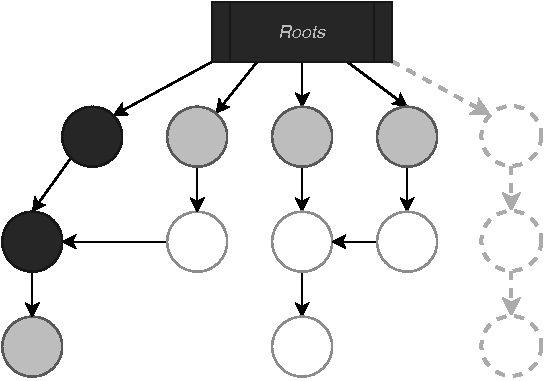
\includegraphics[width=0.4\textwidth]{images/lost-object.pdf}
\end{figure}


Attempts to solve this problem began with Steele~\cite{steele75}, Lamport~\cite{lamport76} and Dijkstra~\cite{dijkstra78}, giving birth to the field of \emph{concurrent garbage collection}. Note that the word concurrent is used in the strict sense here: without loss of generality, we will not consider whether we are trying to run the mutator and the collector in parallel--e.g. on multiple threads--or incrementally by interleaving their execution on a single thread. Instead, we will consider that the mutator and collector both operate in small, atomic operations; and simply look at the way these operations can be interleaved.

When mutator and collector operations become interleaved, the correctness of a garbage collection scheme is both a matter of \emph{safety}--the collector should preserve \emph{at least} all the reachable objects--and \emph{liveness}--every collection cycle should eventually complete. One way to reason about safety is to introduce the concept of \emph{wavefront}: in short, during the marking phase, the traversal can be seen as advancing a wavefront of grey objects, which separate the black objects from the white--unreached--objects. Note that, for the sake of simplicity, we consider here that the object graph contains a special object representing the mutator and pointing to all the mutator roots. Using this waveform abstraction, Wilson observes in~\cite{wilson94} that objects only become lost if the mutator stores a pointer to a white object inside a black object \emph{while} all paths from any grey objects to that white object are destroyed. This leads to the \emph{tricolor invariant}: in order for concurrent collection to be safe, no pointers to white objects must be added to black objects. Intuitively, this means that the collector must be able to assume that once objects become black, it won't need to look at them again during the rest of the cycle. \emph{Note that a weaker version of the tricolor invariant can be formulated, but is it not relevant in the context of this internship.}

Thanks to the special object introduced above, the eventuality of roots being updated during a collection cycle is also taken care of. Depending on the approach used for concurrent collection, this special object will either be given the color grey--meaning that the roots have either not been scanned or might need to be re-scanned--or the color black--meaning that the roots won't need to be scanned anymore.

\subsection{The special case of the Irmin heap}

Instead of digging through the classical techniques for concurrent collection, it is worth remembering that objects in the Irmin heap are immutable. This greatly simplifies the problem of maintaining the tricolor invariant, as concurrent collectors have to deal with the fact that black objects might mutate during a cycle, whereas the only object of the Irmin graph which can mutate during the cycle is the ``special object''--which corresponds to a change of roots, either because a branch was created, updated or deleted. With this in mind, I was able to come up with a relatively simple scheme for concurrent collection in Irmin. It uses a black mutator--meaning that the roots are only scanned once at the beginning of the collection cycle--and a \emph{write barrier}--meaning that the collector will hook into the \texttt{Store} and \texttt{Update} operations of the mutator to avoid breaking the tricolor invariant. \cref{app:concurrent-collection} is a pseudo-code implementation of this scheme.

In this scheme, the special mutator object becomes black at the beginning of the cycle--when \texttt{pending} is filled with \texttt{Roots()}--and stays black during the rest of the cycle. Therefore, to satisfy the tricolor invariant, every outgoing edge added to the mutator object during the cycle must point to a black or a grey object. If the target of that edge was stored during the cycle, it will already be black because of the \texttt{Store} hook, and otherwise it will be colored grey by the \texttt{Update} hook.

Notice that, while it might seem like the \texttt{Update} hook alone would be sufficient to maintain the invariant, the \texttt{Store} hook is needed too: what if an object were stored during a collection cycle, but the cycle finished before the user had time to create a branch referencing it?

Clearly, the time complexity of the marking phase remains unchanged, and the \texttt{Update} and \texttt{Store} hooks are each \(O(1)\). There is no such thing as a free lunch, however, and this concurrent scheme is no exception as it makes two trade-offs to avoid stopping the world. First, it sacrifices some promptness: objects which are stored during a collection cycle but never get referenced by a branch won't get reclaimed until the following cycle; nor will objects which were referenced by a branch at the start of a cycle but become unreachable because the branch gets deleted or updated during the cycle. Second, it can also add some memory overhead to the collection cycle since \texttt{Update} and \texttt{Store} can now add elements to \texttt{pending} and \texttt{marked}. This is usually acceptable, but might become a problem on single-threaded systems if the collector is interleaved with a lot of calls to \texttt{Store}, which might prevent the collector from doing any work while the size of \texttt{marked} grows unbounded.

Finally, astute readers may have noticed that this scheme only really solves part of the concurrency problem since tracing collection is a two-phase process, but we have only allowed concurrent execution of the mutator during the call to \texttt{mark}. To allow it during the entire cycle, we must also ensure that \texttt{backend.heap.Filter} plays nicely with the mutator. Since Irmin backends are modular by design, we don't have control over the concrete implementation of \texttt{Filter}; instead, we update the interface of backends, and require that a call to \texttt{Filter(p)} reclaims objects which do not pass \(p\) only if they have been stored into the backend \emph{before} the call to \texttt{filter}.

\subsection{Implementation details}

The complete implementation of concurrent garbage collection in Irmin is available in \cref{app:concurrent-modular-tracing}.

It is important to note that, in practise, the Irmin mutator and collector both run on the same thread--using the Lwt~\cite{lwt-manual} library for cooperative multitasking--so the execution of their operations is interleaved. First, this means that the problem of unbounded memory mentioned above might apply, so I've had to add a fail-safe which stops the collection cycle and clears \texttt{marked} and \texttt{pending} if their size grows significantly while the collector is unable to progress. Second, this puts us at the mercy of the Lwt scheduler: if the collector doesn't yield back to the scheduler enough; or if the scheduler groups the execution of collector operations without interleaving them with the mutator, the mutator will seem ``stopped'' for a few seconds to an outside observer--the very issue that we were trying to solve. This is particularly dangerous in the case of Tezos, which requires that the mutator always respond in less than a second. To alleviate the issue, I've had to adapt the signature of \texttt{cleanup} to let the caller specify a number of seconds or a number of processed objects after which the collector will be forced to yield back to the mutator, regardless of the scheduling policy of Lwt--as explained on \cref{lst:cleanup-sig}.

\vspace{-.8em}
\begin{figure}[ht]
  \caption{Signature of the \texttt{cleanup} function of Irmin databases.}
  \label{lst:cleanup-sig}

  \centering
  \vspace{-1em}
  \begin{minted}{ocaml}
val cleanup : ?roots:[ `Branches | `List of commit list ] ->
              ?limit_count:int -> ?limit_time:float -> t ->
              (unit, [> `Run_again ]) result Lwt.t
(** [cleanup t] runs the garbage collector on the object graph of database [t].
    Every commit, node and blob which is not reachable from [?roots] will be deleted.

    The garbage collector is concurrent, so collection can safely be interleaved with
    other database operations. This is done via two mechanisms:
    - the Lwt thread of the collector will yield on every I/O operation to allow other
      threads to execute while waiting for results;
    - the [?limit_count] and [?limit_time] options force the collector to return after
      processing more than a set number of objects or after running for a set number 
      of seconds. In this case, the function will return [Error `Run_again], and it
      will need to be run again at a later time to finish collection. *)
    \end{minted}
\end{figure}

\vspace{-1.5em}

As mentioned above, the interface of storage backends--specifically of \texttt{CONTENT\_ADDRESSABLE\_STORE}--must also be updated to mention the additional constraint on \texttt{filter}: a call to \mintinline{ocaml}{filter t p} now informs the content-addressable store that it can remove all values whose key \texttt{k} doesn't satisfy the predicate \texttt{p} \textit{only if they were present in the store before the call to} \texttt{filter}.

There are several ways for backends to handle this additional constraint. A trivial--but somewhat counterproductive--solution is to prevent the storage of new objects into the store during the call to \texttt{filter} altogether by using a lock. A somewhat better solution, which can be applied to every backend, is to allow new objects to be stored during the call to \texttt{filter} but keep track of the hashes of these objects using a set, so that objects get reclaimed only when they don't pass the predicate \emph{and} are not present in the set of recent objects. In some cases--e.g.~when the backend is a single pack-file--there even exist solutions without additional memory overhead; more on this in the chapter on \emph{Backend filtering strategies}.
\newpage

\section{Memory-constrained marking}

Another design goal for our collection scheme is to maintain a \emph{low memory overhead}. This is also particularly important in the Tezos use case, since the memory usage of Irmin inside Tezos nodes is capped at a few hundred megabytes. As mentioned at the end of the chapter on \emph{Garbage collection strategies}, I have used memory profiling tools to cut down on the memory footprint of my collector implementation as much as possible; leaving me with an approximate \(56\) and \(48\) bytes per object hash stored in \texttt{marked} and \texttt{pending} respectively.

With little room left to optimize these figures, I tried to flip the problem around: what if, instead of reducing the footprint of each entry in \texttt{marked} and \texttt{pending}, we reduced the number of entries getting stored there during each collection cycle?

This chapter proposes three strategies that I devised to significantly reduce the number of hashes stored into \texttt{marked} and \texttt{pending} during marking, while still guaranteeing the safety of the collector. While they differ in their specifics, all three are based on the same principle: trading off promptness for space efficiency by implicitly treating a large subset of objects as black regardless of their real color.

\subsection{Partial collection using hash prefixes}

In this first approach, we partition the graph objects into equal-sized subsets based on prefixes of their hashes and run a partial collection cycle for each of these subsets--where each partial cycle only marks objects which belong to its subset, implicitly treating all the other objects as if they were black.

Specifically, let us choose a \emph{prefix length} \(\beta \in \mathbb{N} \cap [1, 256]\), and let us assume that object hashes are distributed uniformly. On a given object graph \(G\), let \(\mu_G\) the maximum amount of memory allocated to the \texttt{marked} set during a collection cycle. We propose a partial collection scheme which allocates at most \(\frac{\mu_G}{2^\beta}\) to \texttt{marked}, but requires \(2^\beta\) complete collection cycles to reclaim all the unreachable objects. Note that, in this scheme, the worst-case runtime of a single collection cycle becomes quadratic in the number of objects in the graph--although this can be alleviated with methods described below.

\cref{alg:partial-prefix} gives a first--naïve--version of the scheme. For the sake of simplicity, we describe the stop-the-world version only--the concurrent one can easily be derived.

\vspace{-.8em}
\begin{figure}[!ht]
  \caption{Naïve partial collection using hash prefixes.}
  \label{alg:partial-prefix}

  \centering
  \begin{lstlisting}
# Run $2^\beta$ partial collection cycles.
atomic Collect($\beta$):
    for prefix in $\{0, 1\}^\beta$:
        marked $\leftarrow$ mark(prefix)
        backend.heap.Filter($\lambda$h. not startsWith(h, prefix) or h $\in$ marked)

# Mark only the objects whose hashes match the given prefix.
mark(prefix):
    # Stack of all the grey objects.
    pending $\leftarrow$ Roots()

    # Set of all the black objects.
    marked $\leftarrow$ $\emptyset$

    while pending $\neq$ $\emptyset$:
        o $\leftarrow$ pop(pending)
        if startsWith(hash(o), prefix) and hash(o) $\not\in$ marked:
            marked $\leftarrow$ marked $\cup$ {hash(o)}
            pending $\leftarrow$ pending $\cup$ successors(o)
        elif not startsWith(hash(o), prefix):
            pending $\leftarrow$ pending $\cup$ successors(o)

    return marked
\end{lstlisting}
\end{figure}

\vspace{-.8em}

As described above, each run of \texttt{mark(prefix)} partitions the objects of \(V\) into two sets \(\Pi\) and \(\bar{\Pi}\) corresponding respectively to the objects whose hashes start with \texttt{prefix} and to the rest. Only objects in \(\Pi\) get added to \texttt{marked} set, while objects in \(\bar{\Pi}\) are all treated as if they were black because of the \texttt{not\ startsWith(h,\ prefix)\ or\ h\ ∈\ marked} predicate. This leaves us with an issue: when we pick an object \(o \in \bar{\Pi}\) from the \texttt{pending} stack, we can't know whether or not we have already traversed \(o\) previoulsy, so we are forced to assume that we haven't. Although this is not critical--remember that the object graph is acyclic, so there is no risk of running into an infinite loop--the worst-case runtime of \texttt{mark} becomes quadratic in the number of objects.

To try to alleviate this issue without increasing the memory usage of the algorithm too dramatically, I added a set of already \texttt{visited} objects implemented using a fixed-sized cache with a \emph{least-recently used} eviction strategy--the size can be adjusted depending on the amount of acceptable memory overhead, with the intuition that a larger cache will usually yield a faster runtime for \texttt{mark}. The choice of the LRU strategy over others--for instance \emph{least-frequently used}--mostly comes down to the fact that it is simple to implement efficiently and has \(O(1)\) insertion and lookup, while most other strategies are more complex and require at least \(O(\log{n})\). The final pseudo-code is given in \cref{app:partial-prefix-lru}.

% TODO: Plot the runtime of the collector when using LRU caches of varying sizes during collection (and update the text).
% TODO: Plot the maximum memory usage of the collector when running partial collection on with varying \beta, versus normally.

\subsection{Partial collection using Bloom filters}

In this other approach, we replace the \texttt{marked} set of objects with a memory-efficient probabilistic set structure called a \emph{Bloom filter}~\cite{bloom70} which lets us known whether an object is either ``possibly black'' or ``definitely white''. Specifically, let us choose a \emph{false positive probability} \(\epsilon \in [0, 1]\). We propose a partial collection scheme which only uses \(m = -\frac{n\ln{\epsilon}}{(\ln{2})^2}\) bits for the \texttt{marked} set, with \texttt{n} the total number of objects in the graph, and which reclaims unreachable objects with probability \(\epsilon\).

\bigskip
Let us start with a quick introduction to Bloom filters. Given \(m \in \mathbb{N}\) a number of bits, and \(k \in \mathbb{N}\) hash functions \((h_i)_{1 \leq i \leq k}\)--which we assume to be independent; a Bloom filter of parameters \((m, k)\) is a probabilistic set data structure which uses a bit array of size \(m\) to answer queries without false negatives. The bit array is initially filled with zeroes; to insert an element \(x\) into the filter in \(O(k)\), we successively compute \(h_1(x), \dots, h_k(x) \in [[1, m]]\) and set the bits at these position in the bit array to \(1\); finally, to test whether or not an element \(y\) is in the filter in \(O(k)\), we also compute \(h_1(y), \dots, h_k(y)\) and return \texttt{false} iff. any of the bits at these position is \(0\)--so we might return false positives, but never false negatives. Assuming that the hash functions are uniform and independent, a quick calculation gives a false positive probability of\(\epsilon = (1 - \frac{1}{m})^k\). Conversely, for a given error probability \(\epsilon\) and an estimated number of elements \(n\), we can compute that the optimal values of \(k\) and \(m\) are \(k = \frac{m}{n} \ \ln{2}\) and \(m = -\frac{n \ln{\epsilon}}{(\ln{2})^2}\).

With this in mind, \cref{app:partial-bloom} gives the pseudo-code for the scheme.

Clearly, since Bloom filters never return false negatives, this scheme is safe--an object can never be treated as white while still being reachable. However, notice that we run into the same problem as the previous scheme: since Bloom filters return false positives, we can never know reliably whether or not we have already traversed a given previously, so we are forced to assume that we haven't. As previously, this means that the worst-case runtime of \texttt{mark} becomes quadratic in the number of objects, but this is somewhat alleviated by the use of a fixed-size LRU cache.

Notice the call to \texttt{newSeed()} when creating the filter, which changes the seed used by the hash functions of the filter at the beginning of each collection cycle. This is done to ensure the completeness of the garbage collection scheme, as there might otherwise exist some unreachable object \(o \in V\) such that \(hash(o)\) always triggers a false positive in the filter; and so it would never get reclaimed. By using a new seed for each cycle, we pick a new set of false positives, and so--assuming uniformity--the probability that an unreachable objects doesn't get reclaimed after \(q\) cycles becomes \(\epsilon^q\).

% TODO: Plot the maximum memory usage of the collector when running partial collection using a Bloom filter with varying percents of accuracy, versus normally.

\subsection{Generational collection}

In this last approach, we draw inspiration from \emph{generational garbage collection} schemes and only reclaim young objects--avoiding older portions of the graph entirely. When used appropriately, this approach can significantly reduce the amount of memory allocated to \texttt{marked} and \texttt{pending} during marking while avoiding the quadratic worst-case runtime and LRU cache of the two previous approaches.

Before describing the scheme in details, let us start with a bit of context. Generational garbage collection is built around the \emph{weak generational hypothesis}--sometimes known as the \emph{infant mortality hypothesis}--which speculates that most objects in a garbage-collected system die young. This hypothesis appears to be valid in the context of memory-managed languages, as demonstrated for example in~\cite{zorn89} for programs written in Common Lisp or~\cite{dieck99} for programs written in Java. Interestingly, this hypothesis also makes intuitive sense in some use cases of Irmin. For instance, most blockchains are designed in such a way that multiple parallel chains of blocks might co-exist for a while, but only the chain with the best score--usually the longest--will eventually become the ``canonical'' chain. Because of this, young blocks which are added to soon-to-be-discarded chains might be broadcasted to all nodes and get stored, only to become quickly unreachable once consensus is reached; whereas old blocks have a greater change of belonging to the ``canonical'' chain, and will likely never become unreachable.

To exploit this idea, we need to define a concept of \emph{object generation}. We say that a function \(\Gamma : H \rightarrow \mathbb{N}\) is a \emph{generation measure} iff. \(\forall o \in V,\ \forall h \in \texttt{successors}(o), \Gamma(\texttt{hash}(o)) \geq \Gamma(h)\). In other words, \(\Gamma\) must preserve the reverse topological ordering of \(G\). Notice that, since the inequality is not strict, a trivial--but not really useful--measure would be the constant \(0\). Intuitively, objects with a small \(\Gamma(o)\) are ``old'', and objects with a large \(\Gamma(o)\) are ``young''.

In practice, Irmin backends will have to provide a generation measure of their choice if they wish to use generational collection. For instance, when the backend is a single append-only pack-file--see the chapter on \emph{Backend filtering strategies} for details--a natural measure is the offset at which the object is stored in the pack-file. Notably, this measure doesn't require any storage overhead, and it is correct because objects in Irmin are immutable, therefore any successor of an object \(o\) must already have been created before it can be referenced in \(o\); meaning that the offset of \(o\) in the pack-file is always greater than the offset of its successors.

With this in mind, let us choose a generation measure \(\Gamma\) as well as an object \(\theta \in V\) called the \emph{threshold}. We propose a partial collection scheme which only traverses the subgraph \(G'\) of reachable objects from \(G\) younger than \(\theta\) according to \(\Gamma\). The \texttt{mark} function runs in \(O(n' + m')\) with \(n'\) the number of objects and \(m'\) the number of edges in \(G'\), and allocates at most \(56\ n'\) bytes of memory for \texttt{marked} and \(48L\) bytes for \texttt{pending} with \(L\) the maximum length of a path in \(G'\). \cref{alg:partial-gen} gives the pseudo-code for this scheme.

\begin{figure}[!ht]
  \caption{Partial collection of objects younger than $\theta$.}
  \label{alg:partial-gen}

  \centering
  \begin{lstlisting}
# Partial collection of objects younger than $\theta$.
atomic Collect($\Gamma$, $\theta$):
    marked $\rightarrow$ mark($\Gamma$, $\theta$)
    backend.heap.Filter($\lambda$h. $\Gamma$(h) < $\Gamma$(hash($\theta$)) or h $\in$ marked)

# Mark the subgraph corresponding to objects younger than $\theta$.
mark($\Gamma$, $\theta$):
    # Stack of all the grey objects.
    pending $\rightarrow$ Roots()

    # Set of all the black objects.
    marked $\rightarrow$ $\emptyset$

    while pending $\neq$ $\emptyset$:
        o $\rightarrow$ pop(pending)
        if $\Gamma$(hash(o)) $\geq$ $\Gamma$(hash($\theta$)) and hash(o) $\not\in$ marked:
            marked $\rightarrow$ marked $\cup$ {hash(o)}
            pending $\rightarrow$ pending $\cup$ successors(o)

    return marked
\end{lstlisting}
\end{figure}


Notice that \texttt{mark} ignores all the paths starting from an object \(o \in V\) as soon as \(\Gamma(\texttt{hash}(o)) < \Gamma(hash(θ))\): this is correct by definition of \(\Gamma\), since any direct or indirect successor \(o'\) of \(o\) will be such that \(\Gamma(\texttt{hash}(o')) \leq \Gamma(\texttt{hash}(o)) < \Gamma(hash(θ))\). This also means that unlike the previous two, this strategy doesn't have a quadratic worst-case runtime nor require an LRU cache, since we can reliably know if we have already traversed an object as long as it is younger than \(\theta\).
\newpage

\section{Backend filtering strategies}

Up until this point in the thesis, we have focused mostly on the marking phase of garbage collection. While this is understandable given that, in our modular collection scheme, the implementation--and thus behavior--of the filtering phase is left to the Irmin backends, this chapter will give a few insights to help the implementation of \texttt{filter} in the non-trivial case of pack-file backends.

\subsection{Pack-file backends}

As mentioned in the introduction, Irmin currently supports several storage backends: \texttt{irmin-mem}, which stores objects in a hashtable in memory; \texttt{irmin-fs}, which persists serialized objects on a POSIX filesystem; \texttt{irmin-git}, which provides a layer of compatibility with Git repositories; and \texttt{irmin-pack}, which persists serialized objects in a single large file similar to a block device.

Since implementing the \texttt{filter} operation is trivial in the case of \texttt{irmin-mem}, \texttt{irmin-fs} and \texttt{irmin-git}, we will exclusively focus on the more complex \texttt{irmin-pack} backend, which was introduced in Irmin 2~\cite{irmin-2-blog} as a way to provide fast and non-blocking access for Irmin objects while reducing the disk footprint of large stores--for instance, the disk usage of Tezos nodes was reduced tenfold after switching from an LMDB-based backend to \texttt{irmin-pack}.

\bigskip
In essence, an instance of \texttt{pack} is a combination of the following elements:
\begin{itemize}
  \item
        The \emph{pack}, shown in \cref{fig:pack}. It is a single append-only file stored on disk which contains a binary encoding--as well as a few bytes of header--of all the objects in the backend. In the algorithms to follow, we will interact with the pack using the following signature:

        \begin{minted}{ocaml}
val read : t -> off:int64 -> bytes -> int
(** [find t ~off b] fills the buffer [b] with the contents of [t] between the
    offsets [off] and [off + size(b)]. Returns the number of bytes read. *)

val offset : t -> int64          (** Returns the current end offset of [t]. *)
val append : t -> string -> unit (** Appends bytes to the end of [t]. *)
val clear : t -> unit            (** Clears the contents of [t]. *)
  \end{minted}
        \vspace{-1em}

  \item
        The \emph{dict}, which is also a single append-only file stored on disk, but is used solely to de-duplicate the names of paths when storing nodes. For the sake of simplicity, we will ignore it in the algorithms to follow--it can be handled like the pack.

  \item
        The \emph{index}, available as a standalone package at~\cite{index-github}. It is a multi-level index persisted on disk, and is used here to associate the hashes of objects with the offset at which they are encoded in the pack. For the sake of brevity, we won't get into details about its implementation; in what follows, we will simply treat it as a black-box with the following signature:

        \begin{minted}{ocaml}
val clear : t -> unit         (** [clear t] removes all the bindings in [t]. *)
val find : t -> key -> value  (** [find t k] is the binding of [k] in [t]. *)
val mem : t -> key -> bool.   (** [mem t k] is [true] iff. [k] is bound in [t]. *)

val replace : t -> key -> value -> unit
(** [replace t k v] binds [k] to [v] in [t], replacing any existing binding of [k]. *)

val iter : (key -> value -> unit) -> t -> unit
(** [iter f t] iterates [f] over the bindings in [t]. *)
  \end{minted}
\end{itemize}

\begin{figure}[ht]
  \caption{Layout of the \texttt{pack} in a pack-file backend.}
  \label{fig:pack}

  \centering
  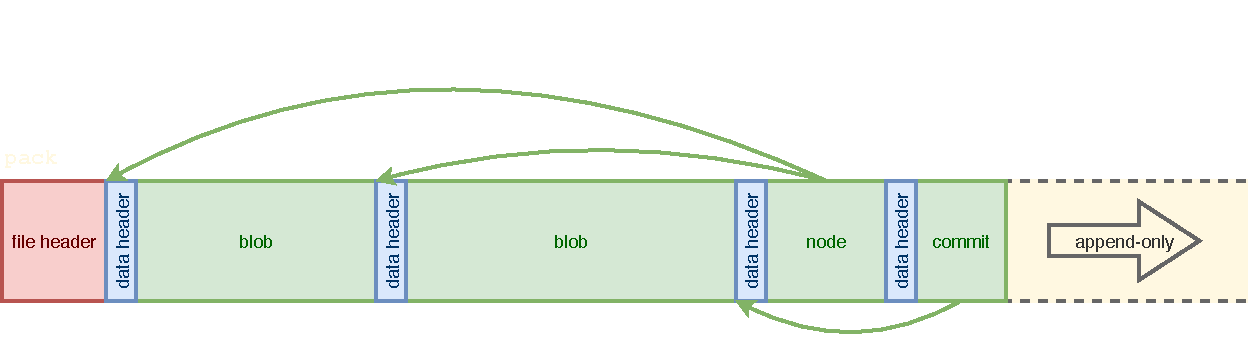
\includegraphics[trim={0 1em 0 3.8em},clip,width=0.85\textwidth]{images/pack.pdf}
\end{figure}


With this in mind, \cref{app:pack-backend} gives a simplified implementation of the \texttt{CONTENT\_ADDRESSABLE\_STORE} interface for a pack-file backend.

\subsection{Copying strategy for pack-file backends}

To implement the \texttt{filter} function in the backend above, I first drew inspiration from the idea of \emph{semispace copying collection} introduced in~\cite{feni69}. In short, copying collectors divide the heap into two equally sized \emph{semispaces}--only one of which is active at any given time. New objects are allocated at the end of the active semispace; and collection can simply be implemented by copying all the marked objects from the active semispace to the other, leaving the unreachable objects behind. The roles of the two semispaces are then switched atomically, and the previously active semispace is reclaimed as a whole--generally by simply resetting its end pointer to the beginning.

Transposing this idea to Irmin, we get the implementation from \cref{app:pack-copying}. It uses two sets of \texttt{Pack.t} and \texttt{Index.t}--one for each semispace. This is equivalent to splitting the pack and the index in two parts, but has the significant advantage that it doesn't require modifying the \texttt{Pack} and \texttt{Index} modules in any way. When \texttt{filter} is called, the backend iterates over all the entries in the current index--i.e.~over all the stored objects--and copies only those which pass the predicate \(p\) to the new index and pack.

This strategy has several advantages: first of all, it is straightforward enough that a bug-free implementation can realistically be produced even when dealing with concurrency or with single-writer multiple-reader parallelism. As mentioned above, it also doesn't require cluttering the behavior of \texttt{Index} and \texttt{Pack} with unrelated concerns. That said, it also has several drawbacks: first, its runtime is proportional to the number--more accurately to the total size--of elements stored in the backend, so calls to \texttt{filter} can quickly get expensive even when there are just a few objects to reclaim. Also, during a call to \texttt{filter}, the disk footprint of the backend can temporarily grow to twice its regular size--which might become a problem for large stores.

\bigskip
A few words about concurrency: as mentioned in the previous chapter on \emph{Concurrent garbage collection}, the responsibility of dealing with concurrency when \texttt{filter} is called is left to the backends. In the implementation above, this is achieved by several means: first, the \texttt{filter} function is wrapped into an Lwt mutex to ensure that it cannot be called while previous calls are still running. As for concurrent calls to \texttt{set} and \texttt{filter}, remember that provides single-threaded cooperative multitasking: we are therefore guaranteed that multiple instructions will execute atomically as long as we don't yield back to the Lwt scheduler between them. In the implementation from \cref{app:pack-copying}, notice that the instructions between lines 85 and 102 never yield back to the scheduler, so the semispace copying is effectively atomic.

While this is generally acceptable, it might become problematic for larger stores--where blocking for the entire duration of the copying process would introduce noticeable mutator pauses. In this case, a solution would be to yield \emph{during} the iteration over \texttt{current\_index}; but we would need a way to make sure that concurrent calls to \texttt{set} don't interfere with the copy. While we could hijack calls to \texttt{set} so that they directly write to the other semispace when \texttt{filter} is running, it is generally not desirable as it might alter the relative ordering of objects in the pack--which we rely on for the generational garbage collection algorithm described above. A better option is to allow calls to \texttt{set} to append to the \texttt{current\_pack} as usual, but to record the end offset \(end\) of the \texttt{current\_pack} at the beginning of the call to \texttt{filter}, and then--during the copying phase--to copy only the objects which pass \(p\) \emph{and} with an offset \(off < end\). Finally, once all such objects are copied, we would block only for the time it takes to copy all the objects with an offset \(off' >= end\)--in other words the objects which were added concurrently.

\subsection{Lazy strategy for pack-file backends}

As mentioned above, the copying implementation of \texttt{filter} has several issues: is that it has a runtime proportional to the number of objects in the store, so it is expensive for large stores even when there are only a few objects to reclaim; and it potentially doubles the disk footprint of the backend for the duration of the call to \texttt{filter}. What follows is an alternative strategy--inspired by the classical mark-and-sweep algorithm--which tries to solve this problem by using switching some of the burden to \texttt{set}.

\bigskip
Precisely, instead of copying all the black objects to another semispace when calling \texttt{filter}, this strategy lazily reclaims the space used by white objects by adding it to a \emph{free list}; such that when \texttt{set} is later called, the backend first tries to allocate new objects into the previously reclaimed space, and falls back to appending at the end of the \texttt{pack} if there is not enough space.

While this strategy has the clear advantage of reducing the runtime and disk overhead of calls to \texttt{filter} dramatically, it comes with two significant trade-offs: first, it can clearly not be used in combination with the generational garbage collection algorithm described in the previous chapter, since the offsets of objects no longer correspond to the time they were added to the pack. More importantly, calls to \texttt{set} are no longer constant-time, but instead have a worst-case runtime of \(O(l)\) with \(l\) the current number of elements in the free list. Although the overhead is usually negligible at first, it might become problematic in the case of \emph{fragmentation}--i.e.~when the free list starts to contain many \((offset, length)\) pairs whose \(length\) is too small to allocate most objects.

How fragmentation evolves over the lifespan of the backend depends mostly on the strategy being used to choose pairs from the free list when allocating an object of size \(length'\): the naive strategy, called \emph{first-fits}, picks the first \((offset, length)\) pair in the list such that \(length >= length'\), removes it from the list, and ``splits'' the corresponding area of memory by putting back \((offset + length', length - length')\) into the list. It should be clear that, when using this strategy, the free-list will become ``polluted'' over time with pairs such that \(length - length'\) is smaller than the size of most objects, leading to a lot a fragmentation. Among the better strategies, \emph{segregated-fits}~\cite{comf64} works by partitioning the set of possible object sizes into arbitrary \emph{size classes}, and uses a free list for each size class instead of a single one. Then, when \texttt{set} tries to find space for an object of size \(length'\), it only has to go through a single free list.

Unfortunately, even if allocation strategies like segregated-fits generally help reduce fragmentation, it can never be fully avoided when free lists are used; and the problem only grows with the number of calls to \texttt{filter} and \texttt{set}. To mitigate the issue, a good compromise is to use the lazy version of \texttt{filter} whenever possible, but to fall back to copying collection whenever fragmentation becomes too important--as a way to compact the ``holes'' in the pack. \cref{app:pack-lazy} provides an implementation of this hybrid strategy. It uses first-fits allocation for the sake of clarity, but can easily be extended to segregated-fits allocation. To keep track of fragmentation, it measures both the number of already reclaimed objects and the ratio between the size of black objects in the pack and the total size of the pack; and it chooses to run the \emph{compacting} version of \texttt{filter} whenever one of these metrics reach a predefined threshold.

Another cause of concern with such a strategy is that writing to the pack-file at random offsets instead of only at its end could have a noticeable runtime overhead. To determine whether this could become a problem, I benchmarked the performance of disk operations on an SSD when using different access patterns and different file modes. The results are available in \cref{app:disk-access}--in short, although there is a noticeable overhead to calling \texttt{seek} then \texttt{write} sequentially when writing at random offsets in a file, it is actually coming from the fact that we are making two system calls rather than from the performance of the disk itself, which can be solved by using the combined \texttt{pwrite} system call instead.

\subsection{Avoiding fragmentation by using interval trees}

Finally, I experimented with ways to significantly reduce the possibility of fragmentation in the previous scheme--so that calls to \texttt{compact\_filter} would no longer be needed. A key insight is to realize that fragmentation can occur for two distinct reasons: either an isolated chunk of the pack was reclaimed, but it is too small for any new object to be allocated in its place; or a large enough portion of the pack is reclaimable, but it is split into many contiguous \((offset, length)\) pairs in the free list--each of them too small to receive a new object. While the first reason is unavoidable, notice that the second one is purely a consequence of the data structure being used: what if, instead of using a free list, we used something more suited to the storage of intervals?

Interestingly enough, there are very few attempts at using structures other than linked lists for allocation in garbage collection literature. This is most likely due to the fact that allocators of memory-managed programming languages are incredibly performance-sensitive, and so the few extra CPU cycles needed to use a more complex data structure are generally prohibitive. In the case of pack-file backends for Irmin, however, this becomes a much more reasonable trade-off--not least because \texttt{set} generally writes to the disk, so the overhead of a few more CPU cycles becomes negligible.

\bigskip
For this experiment, I settled on using an OCaml implementation of Discrete Interval Encoding Trees~\cite{erwig89} available at~\cite{diet-github}, whose abridged signature is given in \cref{app:diet-sig}. Concisely, this data structure uses a binary search tree to store sets of \emph{non-overlapping} discrete intervals. Note that this data structure is \emph{not} an interval tree, since the non-overlapping invariant means that adding \(\llbracket 1, 2 \rrbracket\) to the set \(\{\llbracket2, 3\rrbracket, \llbracket4, 5\rrbracket\}\) will give the set \(\{\llbracket1, 3]], \llbracket4, 5\rrbracket\}\). This would eliminate some fragmentation in free-list backends, since contiguous reclaimed intervals of the pack would be merged together. Let \(n\) be the number of non-overlapping intervals in the DIET. This implementation uses \(O(n)\) storage, and provides \texttt{cardinal} and \texttt{choose} in \(O(1)\) runtime, while \texttt{add} and \texttt{remove} are in \(O(\log{n})\) on average but \(O(n)\) in the worst case.

Given these operations, one can easily write \mintinline{ocaml}{extract : elt -> t -> (interval * t) option} in \(O(n)\), such that \mintinline{ocaml}{extract n t} tries to extract an interval of size \mintinline{ocaml}{n} from \mintinline{ocaml}{t}, and returns either \mintinline{ocaml}{Some (i, rest)} with \mintinline{ocaml}{rest = remove i t} or \mintinline{ocaml}{None} otherwise. It would then be trivial to replace the free list in the strategy above with a DIET which stores a single interval for every non-overlapping chunk of the pack which was previously reclaimed. The implementation of \texttt{filter} would call \texttt{add} every time it finds a white object to reclaim, leading to a \(O(r \log{r})\) runtime when there are \(r\) white objects in the graph--instead of \(O(r)\) when using a free-list. The implementation of \texttt{set} would then call \texttt{extract} with the size of the object to allocate, leading to the same \(O(l)\) runtime as with a free list--with \(l\) the number of intervals in the tree.

Summing up, replacing the free list with a DIET would reduce the fragmentation caused by the free list in the previous strategy at the cost of a \(\log{r}\) factor during calls to \texttt{filter}; which is reasonable given that \texttt{filter} will not be called frequently. To confirm the viability of the strategy, I benchmarked the runtime and storage overhead of DIET operations with a varying number of stored intervals--see \cref{app:diet-bench}. Notice that, even with \(10^4\) intervals in the structure, the runtime of all operations mostly stays an order of magnitude below that of a disk access; so the overhead of the DIET would be negligible.

\section*{Conclusion}
\addcontentsline{toc}{section}{Conclusion}

During my six-month internship at Tarides, I was tasked with the design and implementation of a garbage collection scheme for Irmin, a decentralized database library written in OCaml. I spent the first part of the internship getting familiar with the internals of Irmin--both by submitting general-purpose pull requests to the repository and by implementing a simplified model of Irmin from scratch~\cite{irmin-toy-github}; as well as reviewing garbage collection literature to identify the key concepts and algorithms in the field.

I then tried to adapt some of the ideas from literature into a set of garbage collection schemes that would make sense in the context of Irmin. This was a harder problem than expected, because some usual assumptions about garbage collection in the context of memory-managed programming languages did not apply to Git-based data stores like Irmin.

Eventually, I designed and implemented a \textit{modular} tracing collector which allows different Irmin backends to reclaim unreachable objects differently depending on how they store objects; I designed a simple and efficient \textit{concurrent collection} scheme for Git-based data stores by taking advantage of the immutability of most objects; I tried reducing the memory overhead of garbage collection by proposing several \textit{partial collection} schemes with different time and space trade-offs; and I finally spent some time designing and evaluating different implementations of the \texttt{filter} primitive for pack-like backends.

Future work might include porting some of the schemes I implemented in \texttt{irmin-toy} to \texttt{irmin}--which will require dealing with some of the cross-cutting concerns like single-writer-multiple-reader access. Ideally, work on backend filtering strategies should be continued--notably to try and leverage generational information to reduce the runtime and disk overhead of the copying scheme.

\subsection*{Acknowledgments}

As a closing note, I would like to thank my colleagues at Tarides for their warm welcome, especially given this year's unfortunate turn of events; and Clément, Thomas, Craig and Ioana in particular for their help and guidance on Irmin.

\cref{fig:object-graph} is adapted from \url{https://github.com/CraigFe/git-store-diagram/} by Craig Ferguson, and \cref{fig:pack,fig:dict} are drawn from Clément Pascutto's upcoming ICFP talk on Irmin.

\newpage

\addcontentsline{toc}{section}{References}
\bibliographystyle{abbrv}
\bibliography{bibliography/urls, bibliography/papers}

\newpage

\section*{Appendices}
\addcontentsline{toc}{section}{Appendices}

\vspace{-1.5em}
\titleformat{name=\section}[block]{}{}{0pt}{\colorsection}
\titlespacing*{\section}{0pt}{\baselineskip}{\baselineskip}

\begin{appendices}
  \appendix

  % Prevent the appendices from showing up in the TOC.
  \addtocontents{toc}{\protect\setcounter{tocdepth}{0}}

  \section{Full interface of the \texttt{irmin-toy} library.}
\label{app:irmin-interface}

\setminted{fontsize=\footnotesize,baselinestretch=1}
\inputminted{ocaml}{appendices/sources/s.ml}
  \newpage

  \section{OCaml implementation of modular tracing collection.}
\label{app:modular-tracing}

\setminted{fontsize=\footnotesize,baselinestretch=1}
\begin{minted}{ocaml}
let mark ?(roots = `Branches) t =
  let pending = Stack.create () in
  let marked = OGraph.Table.create 2048 in
  (* Find the entry-points for the graph traversal. *)
  ( match roots with
  | `Branches ->
      (* Lists the commits currently associated to the branches. *)
      Branches.list t >>= fun branches ->
      Lwt_list.map_p (Branches.get_commit_hash t) branches
  | `List commits ->
      (* Lets the user specify a custom list of commits as roots. *)
      commits |> List.map Commits.to_hash |> Lwt.return )
  >|= List.map (fun c -> `Commit c)
  >>= fun entrypoints ->
  let pred = pred ~full:true t in
  let mark key level = OGraph.Table.add marked key level in
  let has_mark key = OGraph.Table.mem marked key in
  (* Add the entrypoints to the set of pending objects. *)
  List.iter (fun k -> Stack.push (k, 0) pending) entrypoints;
  (* Traverse the graph and mark the encountered objects. *)
  let rec visit () =
    match Stack.top pending with
    | exception Stack.Empty ->
        Lwt.return marked
    | key, level ->
        if has_mark key then (
          ignore (Stack.pop pending);
          (visit [@tailcall]) () )
        else (
          incr count;
          mark key level;
          pred key >>= fun keys ->
          List.iter
            (fun (_, k) ->
              if not (has_mark k) then
                Stack.push (k, level + 1) pending)
            keys;
          (visit [@tailcall]) () )
  in
  visit ()

(** [cleanup ~roots t] runs the garbage collector on the object graph of
    database [t]. All the commits, nodes and blobs which are not reachable
    from [roots]–which defaults to all the branches of the database–will be
    deleted from their back-end stores. *)
let cleanup :
    ?roots:[ `Branches | `List of commit list ] -> t -> unit Lwt.t =
    fun ?roots t ->
  (* Start the tracing algorithm, and retrieve the black objects. *)
  Lwt_mutex.with_lock t.write_lock (fun () ->
    mark ?roots t >>= fun marked ->
      (* Filter the stores to keep only the black objects. *)
      Backend.Commits.filter (commits_store t) (fun k ->
          OGraph.Table.mem marked (`Commit (CH (Commit.Digest.serialize k))))
      >>= fun () ->
      Backend.Nodes.filter (nodes_store t) (fun k ->
          OGraph.Table.mem marked (`Node (NH (Node.Digest.serialize k))))
      >>= fun () ->
      Backend.Blobs.filter (blobs_store t) (fun k ->
          OGraph.Table.mem marked (`Blob (BH (Blob.Digest.serialize k)))))
\end{minted}
  \newpage

  \section{Runtime of \texttt{mark} depending on the backend and the number of objects in the heap.}
\label{app:mark-benchmark}

\centering
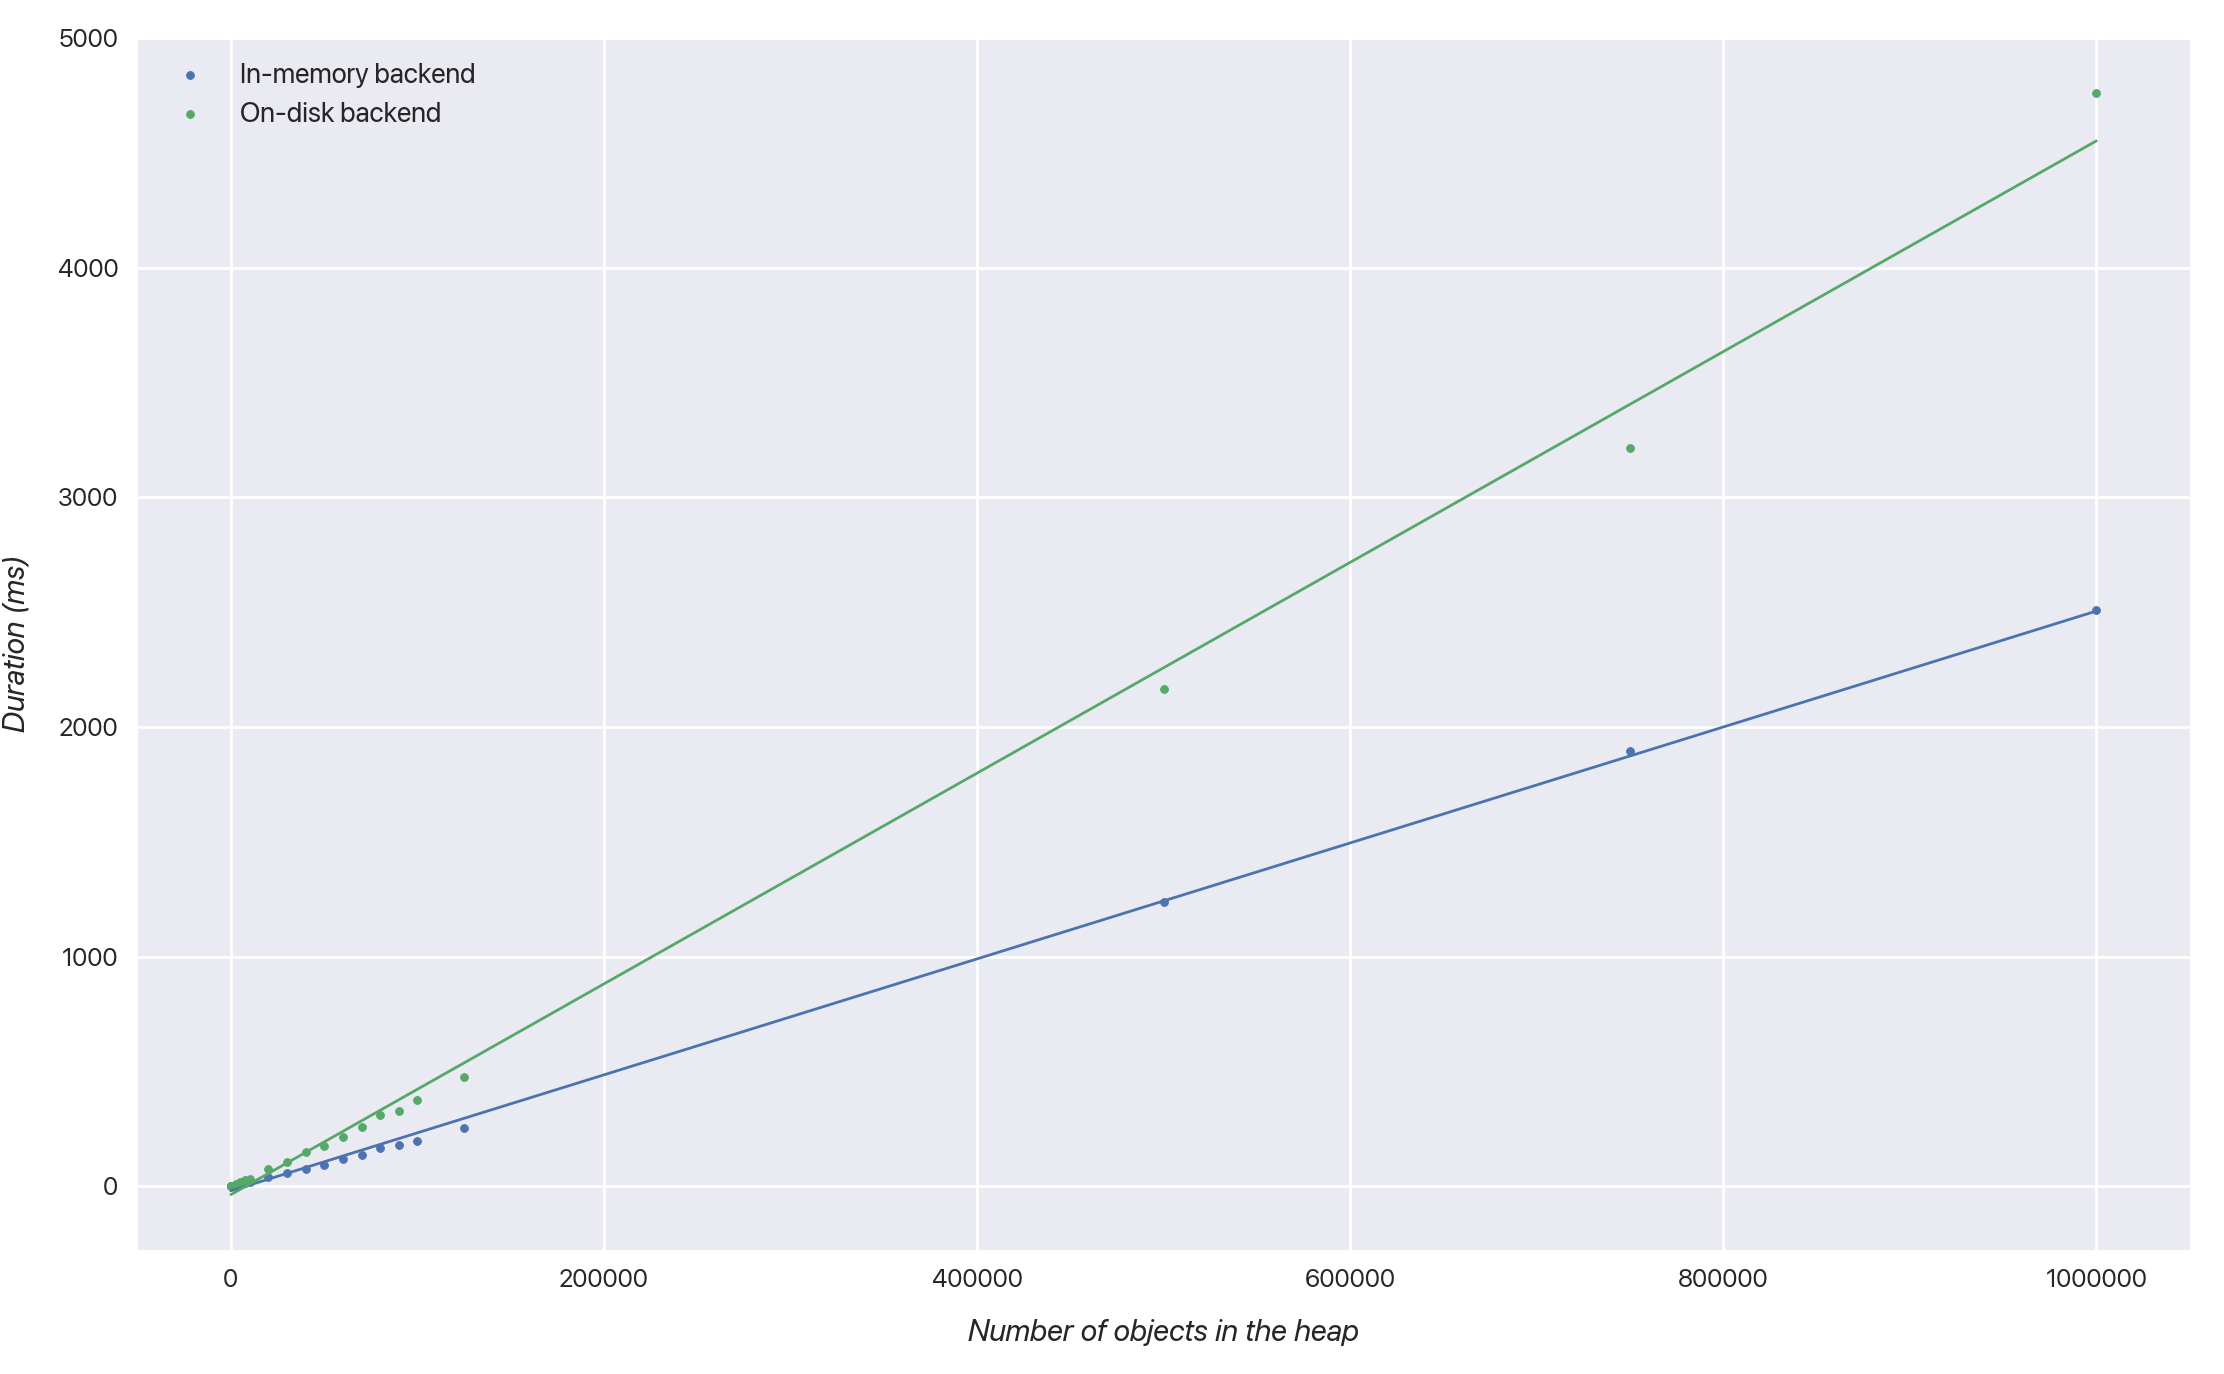
\includegraphics[width=\textwidth]{images/mark_bench.png}

  \newpage

  \section{Pseudo-code implementation of concurrent collection for the Irmin heap.}
\label{app:concurrent-collection}

\centering
\begin{lstlisting}
shared collecting $\leftarrow$ false    # Whether a collection cycle is already active.
shared pending $\leftarrow$ $\emptyset$            # Stack of all the grey objects.
shared marked $\leftarrow$ $\emptyset$             # Set of all the black objects.

# Start a garbage collection cycle.
Collect():
    if collecting:
        raise "Collector is already running."
    prepare()
    mark()
    backend.heap.Filter(λh. h $\in$ marked)
    collecting $\leftarrow$ false

atomic prepare():
    collecting $\leftarrow$ true

    # Reset the object colors.
    pending $\leftarrow$ Roots()
    marked $\leftarrow$ $\emptyset$

mark():
    while pending $\neq$ $\emptyset$:
        visit()

# Atomically pick a grey object and visit it.
atomic visit():
    o $\leftarrow$ pop(pending)
    if hash(o) $\not\in$ marked:
        marked $\leftarrow$ marked $\cup$ {hash(o)}
        pending $\leftarrow$ pending $\cup$ successors(o)

# Store an object on the heap while maintaining the invariant.
atomic Store(o):
    h $\leftarrow$ backend.heap.Set(o)

    # New objects are automatically colored black.
    if collecting:
        marked $\leftarrow$ marked $\cup$ {h}

    return h

# Update a branch while maintaining the invariant.
atomic Update(ref, h):
    backend.refs.Set(ref, h)

    # Targets of branches are automatically colored grey if needed.
    if hash(o) $\not\in$ marked:
        pending $\leftarrow$ pending $\cup$ {hash(o)}
\end{lstlisting}
  \newpage

  \section
    [Simplified implementation of an Irmin database with concurrent tracing collection.]
    {Simplified implementation of an Irmin database with concurrent tracing collection.\\
    \textit{(Elided for readability, full version available at \cite{irmin-toy-database}.)}}
\label{app:concurrent-modular-tracing}

\setminted{fontsize=\footnotesize,baselinestretch=1}
\inputminted{ocaml}{appendices/sources/database.ml}
  \newpage

  \section{Cached partial collection using hash prefixes.}
\label{app:partial-prefix-lru}

\centering
\begin{lstlisting}
# Run $2^\beta$ partial collection cycles.
atomic Collect($beta$):
    for prefix in $\{0, 1\}^\beta$:
        marked <- mark(prefix)
        backend.heap.Filter($\lambda$h. not startsWith(h, prefix) or h $\in$ marked)

# Mark only the objects whose hashes match the given prefix.
mark(prefix):
    marked $\leftarrow$ $\emptyset$           # Set of all the black objects.
    pending $\leftarrow$ Roots()   # Stack of all the grey objects.

    # Fixed-size LRU cache of already visited objects.
    visited <- $\emptyset$

    while pending $\neq$ $\emptyset$:
        o <- pop(pending)
        if startsWith(hash(o), prefix) and hash(o) $\not\in$ marked:
            marked <- marked $\cup$ {hash(o)}
            visited <- visited $\cup$ {hash(o)}
            pending <- pending $\cup$ successors(o)
        elif not startsWith(hash(o), prefix) and hash(o) $\not\in$ visited:
            visited <- visited $\cup$ {hash(o)}
            pending <- pending $\cup$ successors(o)

    return marked
\end{lstlisting}

  \newpage

  \section{Cached partial collection using Bloom filters.}
\label{app:partial-bloom}

\centering
\begin{lstlisting}
# Run a partial collection cycle with false positive probability $\epsilon$.
atomic Collect($\epsilon$):
    marked $\leftarrow$ mark($\epsilon$)
    backend.heap.Filter($\lambda$h. marked.contains(h))

# Mark the objects with false positive probability $\epsilon$.
mark($\epsilon$):
    # Estimate the parameters of the Bloom filter.
    n $\leftarrow$ estimatedObjectCount()
    m $\leftarrow$ ceil(-n * log($\epsilon$) /. log(2 ^ log(2)))
    k $\leftarrow$ ceil(log(2) * m / n)

    # Stack of all the grey objects.
    pending $\leftarrow$ Roots()

    # Set of all the black objects.
    marked $\leftarrow$ newFilter(m, k, newSeed())

    # Fixed-size LRU cache of already visited objects.
    visited $\leftarrow$ $\emptyset$

    while pending $\neq$ $\emptyset$:
        o $\leftarrow$ pop(pending)
        if hash(o) $\not\in$ marked and hash(o) $\not\in$ visited:
            marked.add(hash(o))
            visited $\leftarrow$ visited $\cup$ {hash(o)}
            pending $\leftarrow$ pending $\cup$ successors(o)

    return marked
\end{lstlisting}

  \newpage

  \section{Simplified implementation of a pack-file based \texttt{CONTENT\_ADDRESSABLE\_STORE}.}
\label{app:pack-backend}

\setminted{fontsize=\footnotesize,baselinestretch=1}
\begin{minted}{ocaml}
module Content_Addressable (V : S.HASHABLE) = struct
  module Index = Index.Make
     (struct type t = V.Digest.t end)  (* Use hash digests as keys. *)
     (struct type t = int64 * int end) (* Use (offset, size) pairs as values. *)

  type t = {
    index : Index.t;
    pack : Pack.t;
  }

  type key = V.Digest.t

  type value = V.t

  let mem t k =
    (* An entry is present iff. it is present in the index. *)
    Lwt.return (Index.mem t.index k)

  let find t k =
    (* Find the offset from the index, then read the pack at that offset. *)
    let found =
      match Index.find t.index k with
      | offset, size ->
          let buffer = Bytes.create size in
          let read = Pack.read t.pack ~off:offset buffer in
          if read < size then
            None
          else
            Bytes.unsafe_to_string buffer
            |> V.unserialize
            |> Result.to_option
      | exception Not_found -> None
    in
    Lwt.return found

  let set t v =
    (* Deterministically derive the address of the value. *)
    let h = V.hash v in

    (* Append the bytes to the pack, the update the index. *)
    let offset = Pack.offset t.pack in
    let serialized = V.serialize v in
    let size = String.length serialized in
    Pack.append t.pack serialized;
    Index.replace t.index h (offset, size);
    Lwt.return h
end
\end{minted}
  \newpage

  \section{Simplified implementation of a semispace copying pack-file backend.}
\label{app:pack-copying}

\setminted{fontsize=\footnotesize,baselinestretch=1}
\begin{minted}{ocaml}
module Content_Addressable (V : S.HASHABLE) = struct
  module Index = Index.Make
     (struct type t = V.Digest.t end)  (* Use hash digests as keys. *)
     (struct type t = int64 * int end) (* Use (offset, size) pairs as values. *)

  type t = {
    (* Two atomically switcheable packs for copying garbage collection. *)
    mutable current : [ `A | `B ];
    index_a : Index.t;
    index_b : Index.t;
    pack_a : Pack.t;
    pack_b : Pack.t;
    filter_lock : Lwt_mutex.t;
  }

  type key = V.Digest.t

  type value = V.t

  (** Updates the value of t.current. *)
  let set_current t c =
    (* In a real implementation, the value of current should also be persisted
       to disk so that it can be retrieved when the backend is first opened. *)
    t.current <- c

  (** Returns the [Pack.t] corresponding with [t.current]. *)
  let get_current_pack t =
    match t.current with `A -> t.pack_a | `B -> t.pack_b

  (** Returns the [Pack.t] corresponding with the opposite of [t.current]. *)
  let get_other_pack t = match t.current with `A -> t.pack_b | `B -> t.pack_a

  (** Returns the [Index.t] corresponding with [t.current]. *)
  let get_current_index t =
    match t.current with `A -> t.index_a | `B -> t.index_b

  (** Returns the [Index.t] corresponding with the opposite of [t.current]. *)
  let get_other_index t =
    match t.current with `A -> t.index_b | `B -> t.index_a

  let mem t k =
    (* An entry is present iff. it is present in the index. *)
    let index = get_current_index t in
    Lwt.return (Index.mem index k)

  let find t k =
    (* Find the offset from the current index, then read from the current pack. *)
    let index = get_current_index t in
    let pack = get_current_pack t in
    let found =
      match Index.find index k with
      | offset, size ->
          let buffer = Bytes.create size in
          let read = Pack.read pack ~off:offset buffer in
          if read < size then
            None
          else
            Bytes.unsafe_to_string buffer
            |> V.unserialize
            |> Result.to_option
      | exception Not_found -> None
    in
    Lwt.return found

  let set t v =
    (* Deterministically derive the address of the value. *)
    let h = V.hash v in

    (* Append the bytes to the current pack, the update the current index. *)
    let index = get_current_index t in
    let pack = get_current_pack t in
    let offset = Pack.offset pack in
    let serialized = V.serialize v in
    let size = String.length serialized in
    Pack.append pack serialized;
    Index.replace index h (offset, size);
    Lwt.return h

  let filter t p =
    (* Iterate over all the entries in the current index, and copy all the entries
       that need to be kept to the other index and other pack. Once they are all
       copied, atomically switch [t.current], and finally erase the contents of
       the previous index and pack. *)
    Lwt_mutex.with_lock t.filter_lock (fun () ->
        (* This mutex prevents calls to filter from running concurrently. *)
        let current_index = get_current_index t in
        let other_index = get_other_index t in
        let current_pack = get_current_pack t in
        let other_pack = get_other_pack t in
        let iter k (old_offset, size) =
          (* Only copy entries which satisfy the predicate [p]. *)
          if p k then (
            let buffer = Bytes.create size in
            let read = Pack.read current_pack ~off:old_offset buffer in
            if read < size then invalid_arg "No bytes read."
            else
              let new_offset = Pack.offset other_pack in
              Pack.append other_pack (Bytes.unsafe_to_string buffer);
              Index.replace other_index k (new_offset, size) )
        in
        Index.iter iter current_index;
        set_current t (match t.current with `A -> `B | `B -> `A);
        Lwt_unix.yield () >>= fun () ->
        Index.clear current_index;
        Pack.clear current_pack;
        Lwt.return_unit)
end
\end{minted}
  \newpage

  \section{Simplified implementation of a hybrid pack-file backend.}
\label{app:pack-lazy}

\setminted{fontsize=\footnotesize,baselinestretch=1}
\begin{minted}{ocaml}
module Content_Addressable (V : S.HASHABLE) = struct
  module Index = Index.Make
     (struct type t = V.Digest.t end)  (* Use hash digests as keys. *)
     (struct type t = int64 * int end) (* Use (offset, size) pairs as values. *)

  type t = {
    (* Two atomically switcheable packs for copying garbage collection. *)
    mutable current : [ `A | `B ];
    index_a : Index.t;
    index_b : Index.t;
    pack_a : Pack.t;
    pack_b : Pack.t;
    filter_lock : Lwt_mutex.t;

    (* Mutable set of (offset, size) in the pack that have been reclaimed. *)
    mutable reclaimed : (int64 * int) list;
    mutable reclaimed_count : int64;
    mutable used_pack_size : int64;
    mutable total_pack_size : int64;
  }

  type key = V.Digest.t

  type value = V.t

  (** Updates the value of t.current. *)
  let set_current t c =
    (* In a real implementation, the value of current should also be persisted
       to disk so that it can be retrieved when the backend is first opened. *)
    t.current <- c

  (** Returns the [Pack.t] corresponding with [t.current]. *)
  let get_current_pack t =
    match t.current with `A -> t.pack_a | `B -> t.pack_b

  (** Returns the [Pack.t] corresponding with the opposite of [t.current]. *)
  let get_other_pack t = match t.current with `A -> t.pack_b | `B -> t.pack_a

  (** Returns the [Index.t] corresponding with [t.current]. *)
  let get_current_index t =
    match t.current with `A -> t.index_a | `B -> t.index_b

  (** Returns the [Index.t] corresponding with the opposite of [t.current]. *)
  let get_other_index t =
    match t.current with `A -> t.index_b | `B -> t.index_a

  let mem t k =
    let index = get_current_index t in
    Lwt.return
      ( match Index.find index k with
      (* The offset is -1 when the object has been reclaimed. *)
      | -1L, _ -> false
      (* The object doesn't exist. *)
      | exception Not_found -> false
      | _ -> true )

  let find t k =
    let index = get_current_index t in
    let pack = get_current_pack t in
    let found =
      match Index.find index k with
      | -1L, _ ->
          None (* The offset is -1 when the object has been reclaimed. *)
      | offset, size ->
          let buffer = Bytes.create size in
          let read = Pack.read pack ~off:offset buffer in
          if read < size then None
          else
            Bytes.unsafe_to_string buffer
            |> V.unserialize
            |> Result.to_option
      | exception Not_found -> None
    in
    Lwt.return found

  (** Finds an offset in the pack at which to insert an object of some [size].

      - Starts by looking for space in the list of previously [reclaimed]
        offsets. If such an offset exists, returns [`Offset o]. Note that this
        operation can mutate the [reclaimed] list, e.g. to split a larger block
        of reclaimed memory into two blocks.
      - If no such space is available, returns [`Append] instead. *)
  let allocate t requested_size =
    let first_fits = ref None in
    let find_first_fits (offset, size) =
      if Option.is_some !first_fits then
        Some (offset, size)
      else if size >= requested_size then (
        first_fits := Some offset;
        if size - requested_size > split_threshold then
          Some (offset ++ Int64.of_int requested_size,
                size - requested_size)
        else (
          t.reclaimed_count <- t.reclaimed_count -- 1L;
          None ) )
      else
        Some (offset, size)
    in

    (* Find the first reclaimed region of the pack whose size is sufficient to
       fit the new object, and update the list of reclaimed regions to allow
       splitting regions when necessary. *)
    t.reclaimed <- List.filter_map find_first_fits t.reclaimed;
    t.used_pack_size <- t.used_pack_size ++ Int64.of_int requested_size;
    match !first_fits with
    | None ->
        t.total_pack_size <- t.total_pack_size ++ Int64.of_int requested_size;
        `Append
    | Some offset -> `Offset offset

  let set t v =
    (* Deterministically derive the address of the value. *)
    let h = V.hash v in

    let index = get_current_index t in
    let pack = get_current_pack t in
    let offset = Pack.offset pack in
    let serialized = V.serialize v in
    let size = String.length serialized in

    (* Determine where to store the object in the current pack. *)
    ( match allocate t size with
    | `Offset off -> Pack.set pack ~off serialized
    | `Append ->
        Pack.append pack serialized;
        Index.replace index k (offset, size) );
    Lwt.return_unit

  (** Reclaims the pack storage at [offset..offset+size] used by the object [k]. *)
  let reclaim t k ~offset ~size =
    let index = get_current_index t in
    Index.replace index k (-1L, size);
    t.reclaimed <- (offset, size) :: t.reclaimed;
    t.reclaimed_count <- t.reclaimed_count ++ 1L;
    t.used_pack_size <- t.used_pack_size -- Int64.of_int size

  (** Runs a lazy pass of [filter]. *)
  let lazy_filter t p =
    (* Iterate over all the entries in the current index, and reclaim all those which
       don't need to be kept according to the predicate [p]. *)
    let index = get_current_index t in
    let iter k (offset, size) =
      (* Only reclaim entries which haven't been previously reclaimed (which have an
         offset of -1) and which don't satisfy the predicate [p]. *)
      if offset > -1L && not (p k) then reclaim t k ~offset ~size
    in
    Index.iter iter index;
    Lwt.return_unit

  (** Runs a compaction pass of [filter]. *)
  let compact_filter t p =
    (* Iterate over all the entries in the current index, and copy all the entries
       that need to be kept to the other index and other pack. Once they are all
       copied, atomically switch [t.current], and finally erase the contents of
       the previous index and pack. *)
    let current_index = get_current_index t in
    let other_index = get_other_index t in
    let current_pack = get_current_pack t in
    let other_pack = get_other_pack t in
    let new_pack_size = ref 0L in
    let iter k (old_offset, size) =
      (* Only copy entries which haven't been previously reclaimed (which have an
         offset of -1) and which satisfy the predicate [p]. *)
      if old_offset > -1L && p k then (
        let buffer = Bytes.create size in
        let read = Pack.read current_pack ~off:old_offset buffer in
        if read < size then invalid_arg "No bytes read."
        else
          let new_offset = Pack.offset other_pack in
          Pack.append other_pack (Bytes.unsafe_to_string buffer);
          new_pack_size := !new_pack_size ++ Int64.of_int size;
          Index.replace other_index k (new_offset, size) )
    in
    Index.iter iter current_index;
    t.reclaimed <- [];
    t.reclaimed_count <- 0L;
    t.used_pack_size <- !new_pack_size;
    t.total_pack_size <- !new_pack_size;
    set_current t (match t.current with `A -> `B | `B -> `A);
    Lwt_unix.yield () >>= fun () ->
    Index.clear current_index;
    Pack.clear current_pack;
    Lwt.return_unit

  let filter t p =
    Lwt_mutex.with_lock t.filter_lock (fun () ->
        (* This mutex prevents calls to filter from running concurrently. *)
        if   t.reclaimed_count > reclaimed_threshold
          || t.used_pack_size // t.total_pack_size < loss_ratio_threshold
        then compact_filter t p
        else lazy_filter t p)
end
\end{minted}
  \newpage

  \section{Duration of read and write calls on an SSD using different access patterns \textit{(lower is better)}.}

\label{app:disk-access}
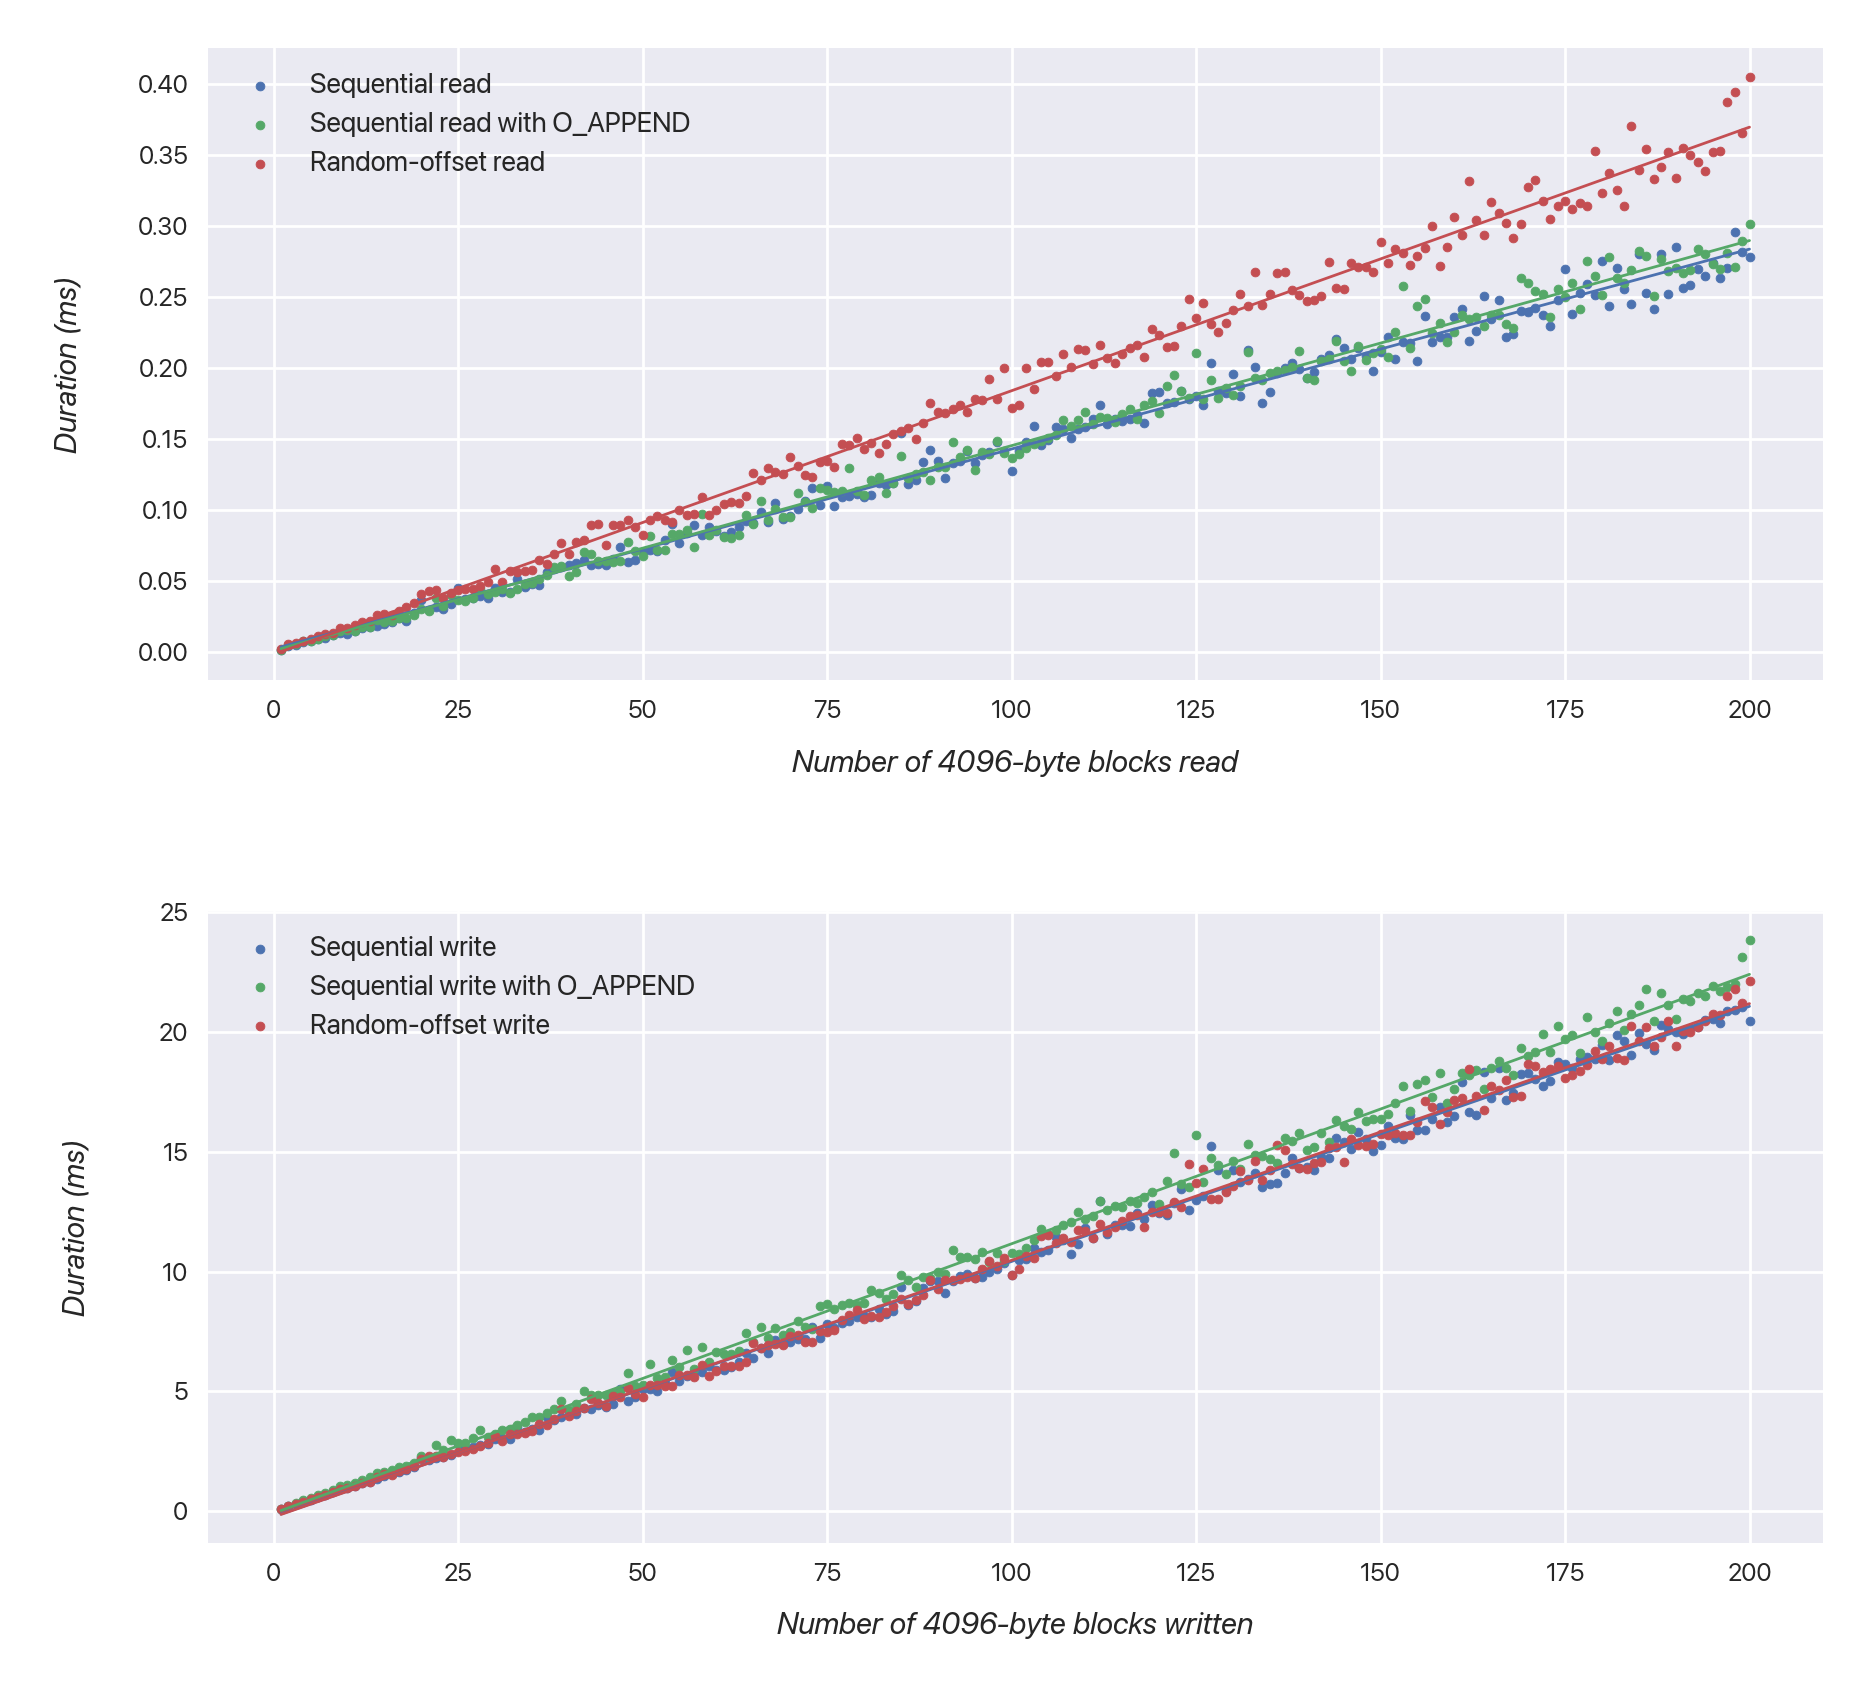
\includegraphics[width=\textwidth]{images/disk_access.png}
  \newpage

  \section{Abridged signature of a DIET interval set.}
\label{app:diet-sig}

\centering
\begin{minted}{ocaml}
module type INTERVAL_SET = sig
  type elt
  (** The type of the set elements *)

  type interval
  (** An interval: a range (x, y) of set values where all the elements from
      x to y inclusive are in the set *)

  type t
  (** The type of sets *)

  val empty: t
  (** The empty set *)

  val cardinal: t -> elt
  (** [cardinal t] is the number of elements in the set [t] *)

  val add: interval -> t -> t
  (** [add interval t] returns the set consisting of [t] plus [interval] *)

  val remove: interval -> t -> t
  (** [remove interval t] returns the set consisting of [t] minus [interval] *)

  val choose: t -> interval
  (** [choose t] returns one interval, or raises Not_found if the set is empty *)
end
\end{minted}

  \newpage

  \section{Runtime and memory benchmark of various DIET operations.}
\label{app:diet-bench}

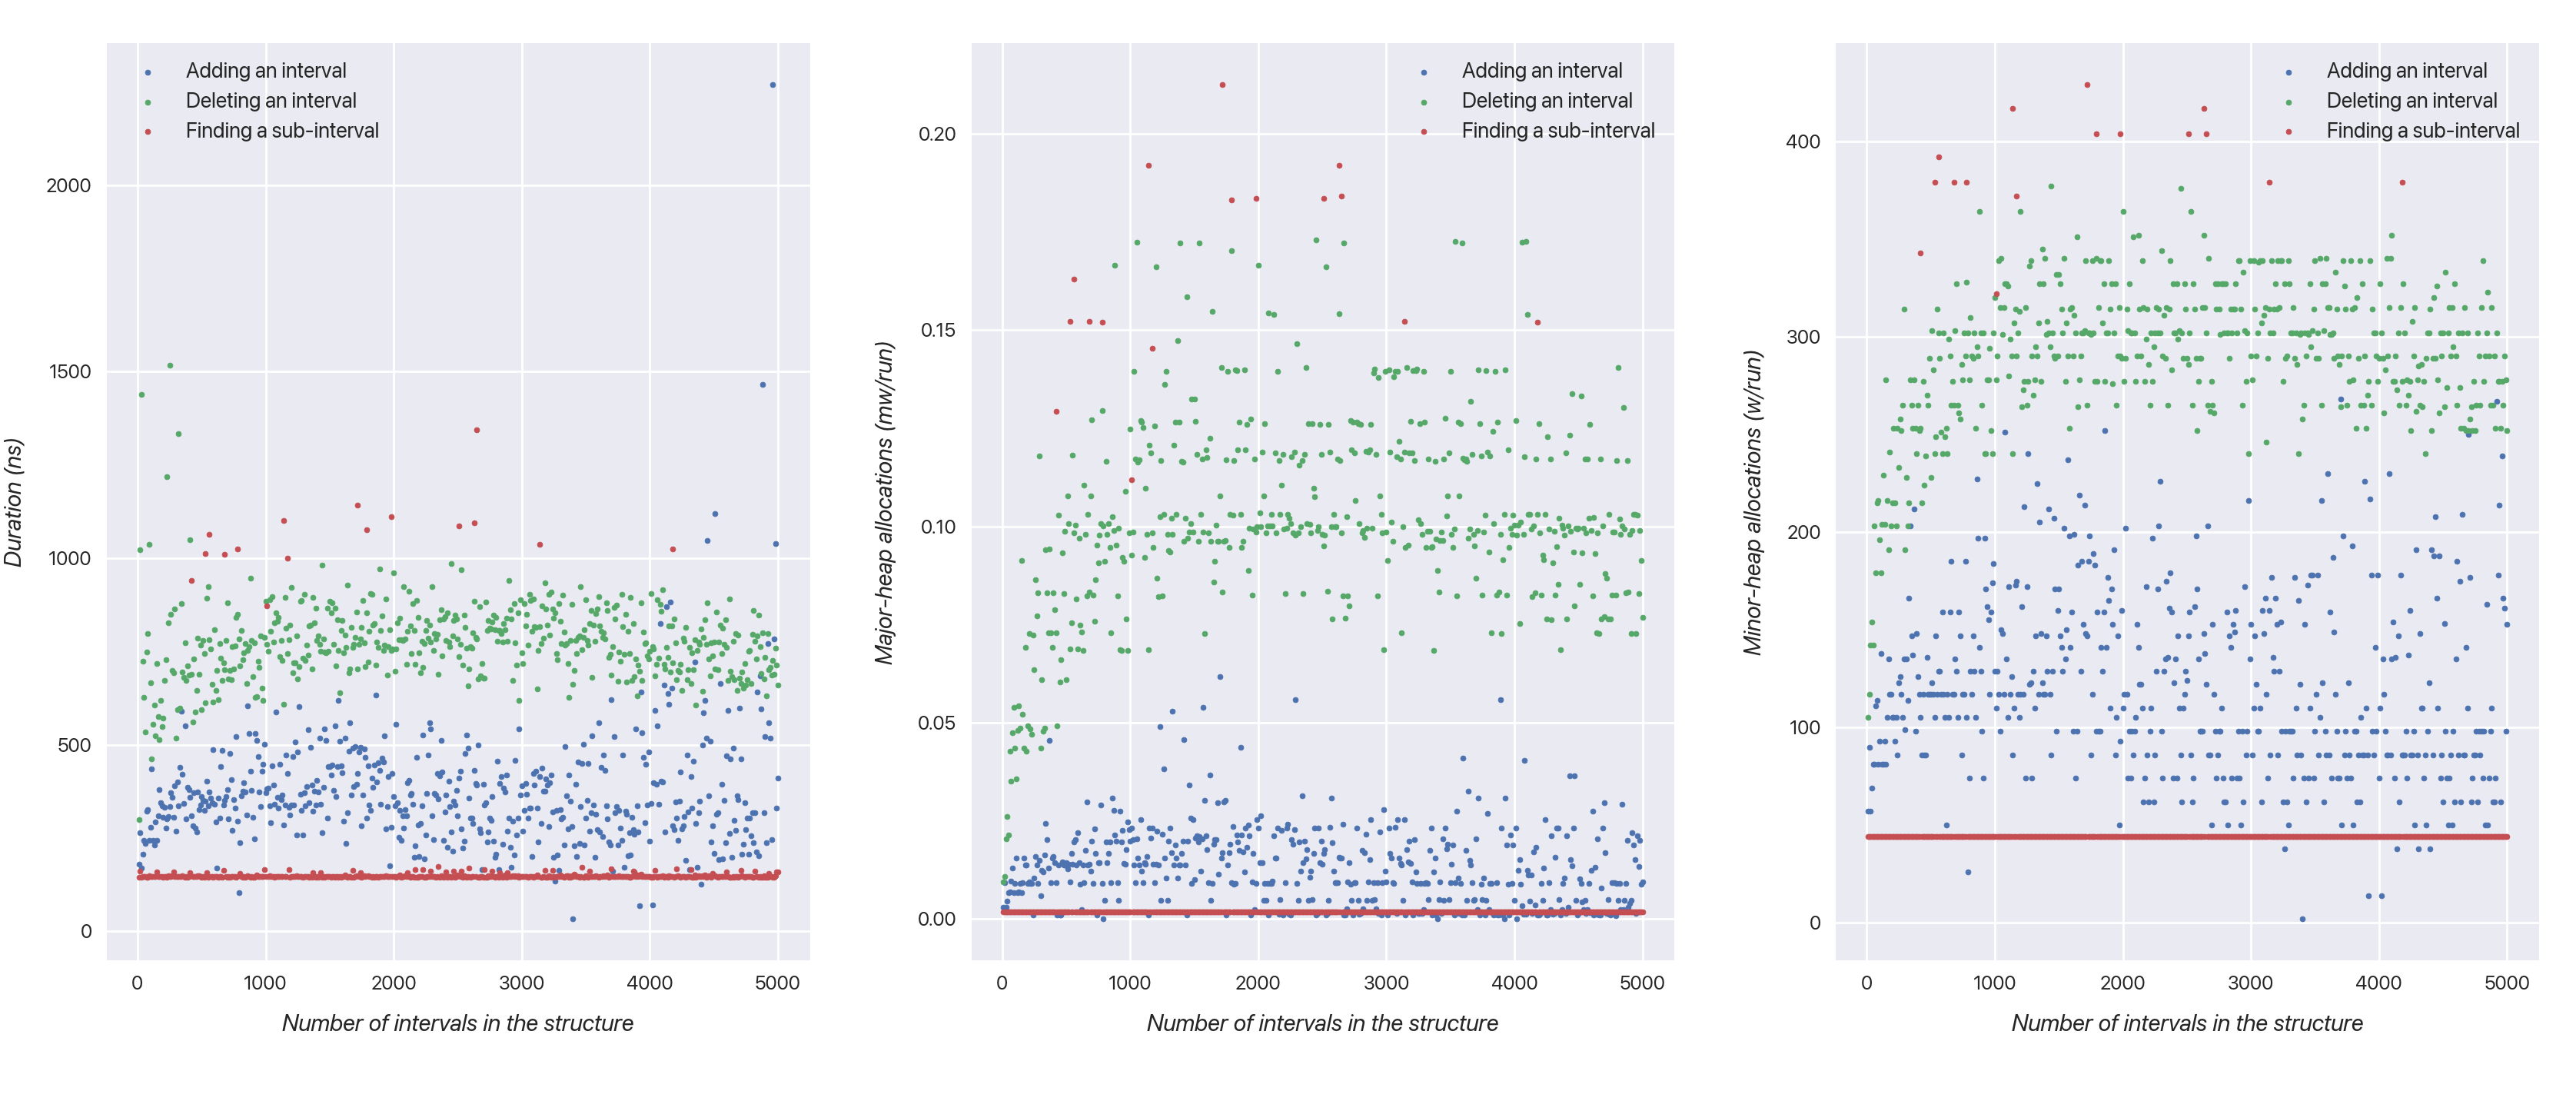
\includegraphics[width=\textwidth]{images/diet_benchs.png}
\end{appendices}


\end{document}
